\documentclass[journal]{IEEEtran}
\usepackage[T1]{fontenc}
\usepackage[utf8]{inputenc}
\usepackage{cite}
\usepackage{amsmath,amssymb}
\usepackage{graphicx}
\usepackage{booktabs}
\usepackage{multirow}
\usepackage{array}
\usepackage{tabularx}
\usepackage{algorithm}
\usepackage{algpseudocode}
\usepackage{url}
\usepackage{xcolor}

\setlength{\textfloatsep}{7pt plus 1pt minus 2pt}
\setlength{\floatsep}{7pt plus 1pt minus 2pt}
\setlength{\intextsep}{7pt plus 1pt minus 2pt}
\setlength{\abovecaptionskip}{3pt}
\setlength{\belowcaptionskip}{0pt}
\setlength{\abovedisplayskip}{5pt plus 1pt minus 2pt}
\setlength{\belowdisplayskip}{5pt plus 1pt minus 2pt}
\renewcommand{\textfraction}{0.08}
\renewcommand{\topfraction}{0.92}
\renewcommand{\dbltopfraction}{0.92}
\renewcommand{\floatpagefraction}{0.8}
\renewcommand{\dblfloatpagefraction}{0.8}
\newcolumntype{Y}{>{\raggedright\arraybackslash}X}
\newcolumntype{L}[1]{>{\raggedright\arraybackslash}m{#1}}
\raggedbottom

\title{Route-Aware Ride-Pooling Dispatch via\\Spatiotemporal Corridor Matching}
\author{Anonymous Authors}

\begin{document}
\maketitle
\vspace{-1.0em}

\begin{abstract}
Ride-pooling studies often evaluate matching after each driver has already been assigned a default route. This paper asks whether scoring a small set of feasible road-network alternatives changes the riders available to a dispatch policy. The proposed matching-ball pipeline requests OSRM alternatives for each driver origin--destination pair, builds route-specific H3 corridors, retrieves riders through coarse spatiotemporal indexing, and then applies exact request-time and route-feasibility checks before route scoring.

The evaluation uses public NYC Yellow and Green Taxi data, with long trips as proxy drivers and shorter trips as proxy rider requests. Riders are pre-sampled to 25\% for offline simulation, indexed with 15-minute H3 bins for retrieval speed, and filtered afterward by an exact request window. In a 60-second rolling-horizon dispatch simulator with rider exclusivity and one-step conflict recomputation, the Yellow 10\% retained-sample scenario gives \(\$8.08\) loss per launched driver under cold-start routing. The strongest non-ML heuristic reduces that loss to \(\$7.30\), ML warm-up reduces it to \(\$7.15\), and the oracle within the route set reaches \(\$7.02\). The same policy ordering appears in the Green same-city service-type check.

A controlled single-driver analysis isolates the route-ranking effect. Across both evaluation layers, strong heuristics recover most of the route-aware gain, while the learned scorer adds a smaller residual improvement. On temporal holdout, the tuned Yellow LightGBM model reaches \(R^2=0.801\) and RMSE \(=\$5.85\); the Green counterpart reaches \(R^2=0.738\) and RMSE \(=\$2.73\). Under this public taxi proxy and fixed economic scenario, route-aware candidate construction changes dispatch outcomes, but learned ranking provides only a modest gain over the strongest rule-based policies.
\end{abstract}

\begin{IEEEkeywords}
ride-pooling, dispatch, route selection, spatiotemporal matching, H3, OSRM, profit prediction, intelligent transportation systems
\end{IEEEkeywords}

\section{Introduction}
\IEEEPARstart{R}{ide}-pooling systems make route and dispatch decisions under tight latency constraints. A common baseline commits each driver to the default route returned by a routing engine, usually the fastest or lowest-cost path. That policy hides a source of variation: two feasible routes between the same endpoints can pass through different rider neighborhoods and therefore expose different time-compatible requests. If the platform scores a small set of road-network alternatives before commitment, route choice becomes part of candidate construction rather than only a navigation detail.

This paper studies that route-choice step through \emph{matching-ball dispatch}. For each driver trip, the platform requests three genuine OSRM alternatives, builds an H3 corridor around each route, retrieves riders whose pickup and drop-off remain compatible with that corridor, and ranks the routes with either rule-based heuristics or a learned route-value model. The design separates retrieval from eligibility. Fifteen-minute H3/time bins narrow the search; riders remain in the candidate set only if their true pickup timestamps satisfy an exact request-offset rule.

The main experiment places route scoring inside a 60-second rolling-horizon dispatch simulator. Active drivers compete for a shared pool of open requests, rider exclusivity is enforced greedily inside each batch, and later drivers are recomputed once against the reduced pool before launch. A larger controlled single-driver study then isolates route-choice effects without dispatch conflict. The two experiments separate the shared-pool question from the route-ranking question.

The main contributions are:
\begin{enumerate}
    \item A timing-aware route-evaluation pipeline that separates coarse H3/time retrieval from exact request-time eligibility.
    \item A route-aware matching-ball method that combines H3 corridor construction, one-ring expansion, exact request filtering, directionality, detour control, and greedy seat assignment into one reproducible retrieval-and-scoring layer.
    \item A dispatch-first evaluation in which route warm-up is embedded inside a 60-second rolling-horizon multi-driver simulator, with a same-city service-type comparison on NYC Yellow and NYC Green Taxi data and an explicit audit of external-city public-data limits.
    \item A baseline study showing that most of the system-level gain comes from route-aware retrieval versus cold-start, while the learned route ranker provides only a modest edge over the strongest non-ML heuristic and a simple path-buffer comparator.
\end{enumerate}

Section II reviews related work. Section III describes the data and proxy construction. Section IV introduces the matching-ball retrieval and route-ranking layer. Section V describes the rolling dispatch simulator. Section VI details the experimental design. Section VII presents system-level and controlled results. Section VIII discusses limitations. Section IX describes code and reproducibility. Section X concludes.

\section{Related Work}
Dynamic ride-sharing and ride-pooling have been studied from the perspectives of assignment, optimization, and feasibility. Alonso-Mora \emph{et al.} cast high-capacity ride-sharing as dynamic trip--vehicle assignment and showed the value of optimization at scale \cite{alonso2017}. Agatz \emph{et al.} surveyed dynamic ride-sharing formulations and emphasized the interaction between temporal constraints and operational trade-offs \cite{agatz2012}; their earlier Atlanta study also showed that better decision rules can outperform naive greedy baselines \cite{agatz2011}. Stiglic \emph{et al.} quantified the role of driver and rider flexibility in dynamic ride-sharing feasibility \cite{stiglic2016}.

Timing assumptions are central in pooling studies. Santi \emph{et al.} quantified shareability under short temporal windows and showed that compatibility assumptions change estimated pooling opportunity \cite{santi2014}. Tachet \emph{et al.} further showed that ride-sharing feasibility scales rapidly with density when the delay window remains small \cite{tachet2017}. Those results motivate our distinction between coarse retrieval bins and exact request-time eligibility.

Ride-hailing dispatch has since grown into a broad literature spanning order assignment, multi-driver coordination, repositioning, and reinforcement learning. Large-platform dispatch has been studied through learning-and-planning formulations \cite{xu2018dispatch,tang2019deepvalue,tang2021value}, while fleet-management and dispatch coordination have also been treated with multi-agent methods \cite{lin2018fleet,zhou2019ovdm,jin2019coride}. Queueing-theoretic dispatch \cite{cheng2019queueing} and practical online repositioning systems \cite{xu2020reposition} further show that system-level outcomes depend on how matching and geographic exposure are coupled over time. More classical pickup-and-delivery and vehicle-routing work \cite{berbeglia2010dynamic,pillac2013dynamic,solomon1987vrptw,savelsbergh1995general} formalizes temporal feasibility and path structure in ways that motivate separating fast retrieval from exact screening. Complementary fleet-scale and stochastic views \cite{vazifeh2018fleet,bertsimas2019online,ozkan2020dynamic,braverman2019empty} emphasize supply--demand imbalance, idle routing, and online matching under uncertainty. Recent ride-pooling traffic and pricing studies \cite{ke2020ridepooling,karaenke2023expool} connect these operational rules to congestion and revenue management. Our paper does not attempt to replace that broader fleet-optimization literature. It focuses on a narrower question that those studies usually absorb into a larger optimizer: whether route choice itself changes the candidate pool enough to affect dispatch outcomes.

Route recommendation has also been studied as a matching-quality lever rather than only a routing problem. Ma \emph{et al.} developed T-Share, a large-scale dynamic taxi ridesharing service with spatiotemporal indexing \cite{ma2013tshare}. Later work explored route recommendation for carpool facilitation \cite{bassem2022}, route-aware matching over joint social and road networks \cite{xia2019}, and search-based online decision improvement \cite{chen2021}. More recent formulations push toward jointly optimizing matching, routing, and pickup/drop-off design in rolling-horizon settings \cite{stumpe2024}. Those studies motivate our route-aware formulation, but our methodological emphasis is different: we separate route-aware candidate construction from exact-time eligibility and ask how much of the resulting lift survives inside a lightweight dispatch layer.

Recent ride-hailing work has also highlighted fairness and system design concerns beyond pure efficiency \cite{suhr2019fair,shi2021fair,raman2021fair}. We do not model fairness or repositioning explicitly here, and we therefore avoid claiming a full fleet-management solution. Instead, the paper contributes a reproducible public-data benchmark for route-aware candidate construction under realistic timing assumptions.

Methodologically, the implementation uses H3 spatial indexing \cite{h3docs}, OSRM route alternatives \cite{osrmapi}, and gradient-boosted trees via LightGBM \cite{ke2017} and XGBoost \cite{chen2016xgboost}, with comparison baselines that include a linear regressor, LambdaRank, and a neural network. The novelty is therefore not ``use ML on taxi data,'' but to combine route-aware retrieval, exact request timing, and system-level dispatch evaluation in one reproducible workflow. Table~\ref{tab:prior_work_positioning} makes that positioning explicit: we reuse proven indexing, routing, and learning components, and contribute the route-specific candidate-construction/evaluation layer rather than a new global fleet optimizer.

\begin{table*}[!t]
\caption{Positioning relative to closely related ride-pooling and dispatch literature.}
\label{tab:prior_work_positioning}
\centering
\footnotesize
\begin{tabularx}{\textwidth}{|L{0.20\textwidth}|L{0.24\textwidth}|L{0.29\textwidth}|Y|}
\hline
Literature family & Reused or related idea & Paper-specific contribution & Scope boundary \\
\hline
T-Share / dynamic taxi ridesharing & Spatiotemporal indexing and dynamic matching & Public-data route-corridor exposure with exact post-retrieval eligibility & We do not reproduce T-Share fleet optimization; we compare the route-retrieval primitive and dispatch-lite layer. \\
\hline
Shareability networks & Compatibility under time and delay windows & Route-specific candidate-pool construction over OSRM alternatives & Shareability is an inspiration, not a direct optimization baseline. \\
\hline
Dynamic trip--vehicle assignment & Global assignment over requests and vehicles & Low-latency route-choice layer before assignment & The simulator is not a replacement for RTV/global optimization. \\
\hline
Rolling-horizon dispatch studies & Batching and online reassignment & 60-second shared-request route-choice evaluation & We add rider exclusivity but not repositioning or long-horizon fleet control. \\
\hline
Path-buffer/geometric retrieval & Simple route-neighborhood exposure & H3 pickup-and-drop-off corridor eligibility plus exact timing & Included as a bounded sanity baseline, not as a state-of-the-art dispatch optimizer. \\
\hline
Learning-based dispatch/ranking & ML value estimation or order assignment & Learned route ranking after explicit candidate construction & ML is a residual scorer, not the primary source of lift. \\
\hline
\end{tabularx}
\end{table*}

\section{Data and Proxy Construction}
\subsection{Public Domains}
We use the NYC Yellow Taxi and NYC Green Taxi public datasets from Azure Open Datasets \cite{azureyellow,azuregreen,azuredocs}. The retained columns include trip timestamps, pickup and drop-off coordinates, trip distance, fare amount, total amount, tips, and passenger count. Table~\ref{tab:data_split} summarizes the temporal split: January--February 2015 are used for training, March 2015 for temporal validation and model selection, and April 2015 for policy evaluation. Green data are used as a public same-city service-type check rather than as evidence from a second city.

We audited major public external-city candidates before choosing this scope. Chicago TNP/Taxi is the strongest candidate because it includes trip-level OD centroids, timestamps, distance, and rounded fare, but its privacy rounding changes both corridor geometry and exact-time matching. Porto taxi trajectories preserve GPS trajectories but lack comparable fare fields for the scenario-profit model. Washington DC and major-city portals including San Francisco, Los Angeles, Austin, Seattle, Toronto, Boston, Philadelphia, Dallas, and Houston expose either coarser geography, aggregate mobility products, or no comparable official taxi/TNC OD table. Table~\ref{tab:external_data_audit} summarizes the decision; the paper therefore reports Green as same-city service-type evidence and treats true external-city validation as future work rather than as an unsupported result.

\begin{table}[!t]
\caption{Temporal split used in both public domains.}
\label{tab:data_split}
\centering
\footnotesize
\begin{tabularx}{\columnwidth}{|L{0.18\columnwidth}|L{0.28\columnwidth}|Y|}
\hline
Role & Months & Purpose \\
\hline
Training & January--February 2015 & Model fitting and historical summaries \\
\hline
Validation & March 2015 & Temporal holdout selection and calibration \\
\hline
Evaluation & April 2015 & Dispatch and paired-policy experiments \\
\hline
\end{tabularx}
\end{table}

\begin{table*}[!t]
\caption{External public-data audit used to scope the same-city service-type comparison.}
\label{tab:external_data_audit}
\centering
\footnotesize
\begin{tabularx}{\textwidth}{|L{0.20\textwidth}|L{0.29\textwidth}|L{0.27\textwidth}|Y|}
\hline
Candidate & Relevant fields & Limitation for this paper & Decision \\
\hline
Chicago TNP/Taxi & Trip-level OD centroids, timestamps, distance, rounded fare, shared-trip fields & Coordinates and fares are privacy-rounded; exact-point route corridors are not directly comparable & Best future external-city candidate; do not mix with NYC exact-point claims without a separate method section. \\
\hline
Porto taxi trajectories & GPS OD/trajectory and start timestamp & No comparable public fare/economic field for the scenario-profit model & Useful for route mechanics only; excluded from profit dispatch evidence. \\
\hline
Washington DC taxi & Public taxi records with coarse OD/time fields & Hour/block-level rounding is too coarse for exact request-window matching & Excluded from primary evaluation. \\
\hline
NYC HVFHV/FHV & Native ride-hailing context and timestamps & Taxi-zone IDs rather than point coordinates; not an external city & Future native ride-hailing extension, not external-city evidence here. \\
\hline
San Francisco, Los Angeles, Austin, Seattle, Toronto, Boston, Philadelphia, Dallas, Houston portals & Major municipal open-data portals & No clean official trip-level taxi/TNC OD release comparable to NYC/Chicago found in the audit & Do not force weak evidence; soften external-city claims. \\
\hline
\end{tabularx}
\end{table*}

\subsection{Proxy Roles and Retained-Sample Semantics}
Trips are partitioned into:
\begin{itemize}
    \item \textbf{Drivers:} trips longer than 10 miles.
    \item \textbf{Riders:} trips from 0.5 to 10 miles.
\end{itemize}

Riders are pre-sampled to 25\% before any density sweep. This is a tractability choice for the public benchmark, not a claim about full market share. Throughout the paper, \emph{100\% density} therefore means the full retained 25\% rider sample, not full city demand. We also report a retained-sample sensitivity over 10\%, 25\%, and 100\% of that fixed rider pool, corresponding approximately to 2.5\%, 6.25\%, and 25\% of the full extracted rider population. This check does not replace a fresh raw-data extraction at different pre-sampling probabilities, but it shows that the route-aware ordering is not an artifact of a single active-rider density.

Table~\ref{tab:proxy_distribution} reports the retained role sizes and distance distributions after the proxy split. The processed analysis files support exact sensitivity counts for driver thresholds at or above 10 miles and rider thresholds up to 10 miles. Wider sensitivity points outside those retained files require rerunning raw extraction, so they are reported in the reproducibility materials as audit notes rather than treated as observed counts.

\begin{table}[!t]
\caption{Proxy role counts and retained distance distributions. Rider counts are the retained 25\% sample.}
\label{tab:proxy_distribution}
\centering
\scriptsize
\setlength{\tabcolsep}{3.0pt}
\begin{tabular}{|l|l|r|r|r|r|}
\hline
Split & Role & Rows & P25 mi & Median mi & P75 mi \\
\hline
Train & Driver & 1{,}800{,}319 & 11.31 & 14.50 & 17.80 \\
\hline
Train & Rider & 8{,}084{,}705 & 1.12 & 1.77 & 2.97 \\
\hline
Test & Driver & 668{,}476 & 11.31 & 14.60 & 17.81 \\
\hline
Test & Rider & 2{,}759{,}327 & 1.16 & 1.80 & 3.02 \\
\hline
\end{tabular}
\end{table}

\subsection{Proxy Validity and Scope}
The retained taxi trips are not native pooled requests, and the platform-side economics do not encode rider acceptance, cancellation, or driver repositioning behavior. The proxy is useful for the narrower question studied here because it preserves exact pickup/drop-off coordinates, timestamps, trip distances, and fare magnitudes at city scale under a public benchmark. It supports relative comparison of route-aware candidate construction, exact-time eligibility, and route-ranking policies under controlled assumptions. It does not support claims about market adoption, platform-wide profitability, or behavioral response to pooling incentives.

\subsection{Scenario Assumptions}
Reported values are \emph{scenario profit} outputs under fixed assumptions. Table~\ref{tab:scenario_assumptions} summarizes the primary configuration and the sensitivity ranges used later in the paper. Table~\ref{tab:economics_sensitivity} reports the corresponding economic sensitivity for the 10\% single-driver setting. These settings support controlled comparison; they are not calibrated platform margins.

\begin{table}[!t]
\caption{Scenario assumptions and operating regimes used throughout the paper.}
\label{tab:scenario_assumptions}
\centering
\footnotesize
\begin{tabularx}{\columnwidth}{|L{0.26\columnwidth}|L{0.22\columnwidth}|Y|}
\hline
Component & Primary value & Notes / sweep \\
\hline
Indexing cadence & 15-minute bins, \(\pm1\) adjacent bins & Retrieval only; not the final eligibility rule \\
\hline
Exact request window & 5 minutes & Sensitivity: \(\{2,5,10\}\) minutes \\
\hline
Maximum detour & 4 minutes & Sensitivity: \(\{2,4,6\}\) minutes \\
\hline
Retained-sample density & 10\% headline sparse regime & Density sweep: \(\{100,25,10\}\)\% of the pre-sampled rider pool \\
\hline
Seat capacity & 3 seats per driver & Fixed across all experiments \\
\hline
Platform share & \(\alpha=0.50\) & Scenario-profit assumption \\
\hline
Driving cost & \(c=\$0.67\) per mile & Scenario-profit assumption \\
\hline
Urban speed proxy & 40 km/h & Converts geometric detour into minutes \\
\hline
\end{tabularx}
\end{table}

\begin{table}[!t]
\caption{Single-driver economic sensitivity at 10\% retained density. Values are scenario profit per driver under ML warm-up, not calibrated platform margins.}
\label{tab:economics_sensitivity}
\centering
\scriptsize
\setlength{\tabcolsep}{4.0pt}
\begin{tabular}{|l|r|r|r|}
\hline
Scenario & Share \(\alpha\) & Cost/mi & Profit/driver \\
\hline
Primary & 0.50 & 0.67 & -6.17 \\
\hline
Lower share & 0.40 & 0.67 & -7.05 \\
\hline
Higher share & 0.60 & 0.67 & -5.28 \\
\hline
Lower cost & 0.50 & 0.50 & -5.46 \\
\hline
Higher cost & 0.50 & 0.85 & -6.94 \\
\hline
\end{tabular}
\end{table}

\begin{figure*}[!t]
\centering
\includegraphics[width=\textwidth]{figures/paper_fig1_dispatch_architecture_v2.png}
\caption{Dispatch-first system architecture. The figure separates offline asset construction from online route scoring and from the two evaluation branches used in the paper. The key methodological distinction is that H3 corridors and 15-minute bins are used only to narrow the search, whereas exact request compatibility and route feasibility are enforced afterward before policy scoring.}
\label{fig:dispatch_architecture}
\end{figure*}

\section{Matching-Ball Retrieval and Route Ranking}
Figure~\ref{fig:dispatch_architecture} summarizes the paper's end-to-end pipeline, and Table~\ref{tab:notation} collects the notation used throughout this section. Public taxi trips are converted into proxy drivers and riders, each driver receives three genuine route alternatives, matching-ball retrieval narrows the candidate pool through H3 corridors and coarse time bins, and exact request compatibility is enforced only after retrieval. The resulting route scores then feed both the rolling dispatch simulator and the larger single-driver paired study.

\begin{table}[!t]
\caption{Notation used in the matching-ball and dispatch formulation.}
\label{tab:notation}
\centering
\footnotesize
\begin{tabularx}{\columnwidth}{|L{0.30\columnwidth}|Y|}
\hline
Symbol & Meaning \\
\hline
\(d \in \mathcal{D}\) & Driver trip in the evaluation set \\
\hline
\(u \in \mathcal{U}\) & Rider request \\
\hline
\(\mathcal{R}_d=\{r_{d1},\dots,r_{dK}\}\) & Candidate route set for driver \(d\), with \(K=3\) in the paper \\
\hline
\(\pi_r\) & Polyline of route \(r\) returned by OSRM \\
\hline
\(R_r\) & Ordered H3 spine obtained by densifying \(\pi_r\) and mapping it to H3 cells \\
\hline
\(C_r\) & Matchable H3 corridor derived from \(R_r\) \\
\hline
\(h_u^{p}, h_u^{q}\) & Pickup and drop-off H3 cells of rider \(u\) \\
\hline
\(t_d, t_u\) & Driver departure timestamp and rider pickup timestamp \\
\hline
\(\tau_{\mathrm{req}}, \tau_{\mathrm{det}}\) & Exact request-time and detour thresholds \\
\hline
\(\mathcal{U}_r^{\mathrm{cand}}, \mathcal{U}_r^{\mathrm{feas}}\) & Retrieved candidate set and exact-feasible rider set for route \(r\) \\
\hline
\(M_r\) & Matched rider set produced for route \(r\) after greedy seat assignment \\
\hline
\(s_\phi(d,r)\) & Route score under policy \(\phi\) \\
\hline
\(g(d,r)\) & Realized scenario profit for assigning driver \(d\) to route \(r\) \\
\hline
\(\mathcal{U}_b\) & Open request pool at dispatch batch \(b\) \\
\hline
\end{tabularx}
\end{table}

\subsection{H3 Corridor Construction}
Each driver origin--destination pair is routed through OSRM \cite{osrmapi}. The implementation stores a persistent route cache so that evaluation does not depend on live API latency once the cache is populated. For each driver \(d\), three genuine road-network alternatives are requested. Every route polyline \(\pi_r\) is densified at 80 m spacing and mapped to ordered H3 resolution-9 cells \cite{h3docs}. Let \(R_r=(h_1,\dots,h_m)\) denote the ordered H3 cells traversed by route \(r\). The matchable corridor is
\[
C_r=\bigcup_{h\in R_r}\mathrm{Disk}_{\kappa}(h),
\]
where \(\mathrm{Disk}_{\kappa}(h)\) is the H3 \(\kappa\)-ring neighborhood around cell \(h\). The primary configuration uses \(\kappa=1\), i.e., \(\mathrm{Disk}_1(h)\); later sensitivity analysis varies corridor width to show how retrieval geometry changes both the candidate pool and the ranking difficulty.

\subsection{Exact-Time Matching-Ball Retrieval}
Retrieval is intentionally two-stage. Each rider is indexed by pickup cell, drop-off cell, service date, and 15-minute pickup bin. At query time, the route contributes its corridor cells \(C_r\), and the retrieval step searches the driver's departure bin plus adjacent bins on the same service date only as a coarse speed device. The coarse candidate set for route \(r\) is
\begingroup
\small
\begin{equation}
\mathcal{U}_r^{\mathrm{cand}}=
\left\{
u\in\mathcal{U}\ \middle|\
\begin{aligned}
&h_u^{p}\in C_r,\ h_u^{q}\in C_r,\\
&\beta(t_u)\in\{\beta(t_d)-1,\beta(t_d),\beta(t_d)+1\},\\
&\delta_u=\delta_d
\end{aligned}
\right\}.
\end{equation}
\endgroup
Here \(\beta(\cdot)\) maps a timestamp to its 15-minute bin and \(\delta_u\) is the service date. Exact eligibility is then enforced on the true pickup timestamp:
\[
|t_u - t_d| \le \tau_{\mathrm{req}},
\]
with \(\tau_{\mathrm{req}}=5\) minutes in the primary scenario.

The exact-feasible set is therefore
\begingroup
\small
\begin{equation}
\mathcal{U}_r^{\mathrm{feas}}=
\left\{
u\in\mathcal{U}_r^{\mathrm{cand}}\ \middle|\
\begin{aligned}
&|t_u-t_d|\le\tau_{\mathrm{req}},\\
&\psi_r(u)=1,\ \Delta_r(u)\le\tau_{\mathrm{det}},\\
&p_u\le s_d
\end{aligned}
\right\}.
\end{equation}
\endgroup
Here \(\psi_r(u)\) is a directionality-validity indicator, \(\Delta_r(u)\) is detour in minutes, \(p_u\) is rider party size, and \(s_d\) is remaining seat capacity. Matching-ball retrieval is therefore route-aware, date-aware, and exact-time eligible even though coarse bins are used for indexing speed.

Operationally, \(\psi_r(u)\) is computed by projecting the rider pickup and drop-off points onto the candidate route polyline and requiring the normalized drop-off projection to be downstream of the pickup projection by at least 0.05 of the route length. The detour term \(\Delta_r(u)\) is a geometric proxy: the pickup and drop-off perpendicular distances to the route are doubled, inflated by a 1.3 Manhattan factor, and converted to minutes with the 40 km/h scenario speed. Multiple riders are handled after this filter by sorting feasible riders by platform fare share, adding seed-controlled tie-breaking noise, and filling seats greedily until the three-seat capacity is exhausted.

\begin{figure*}[!t]
\centering
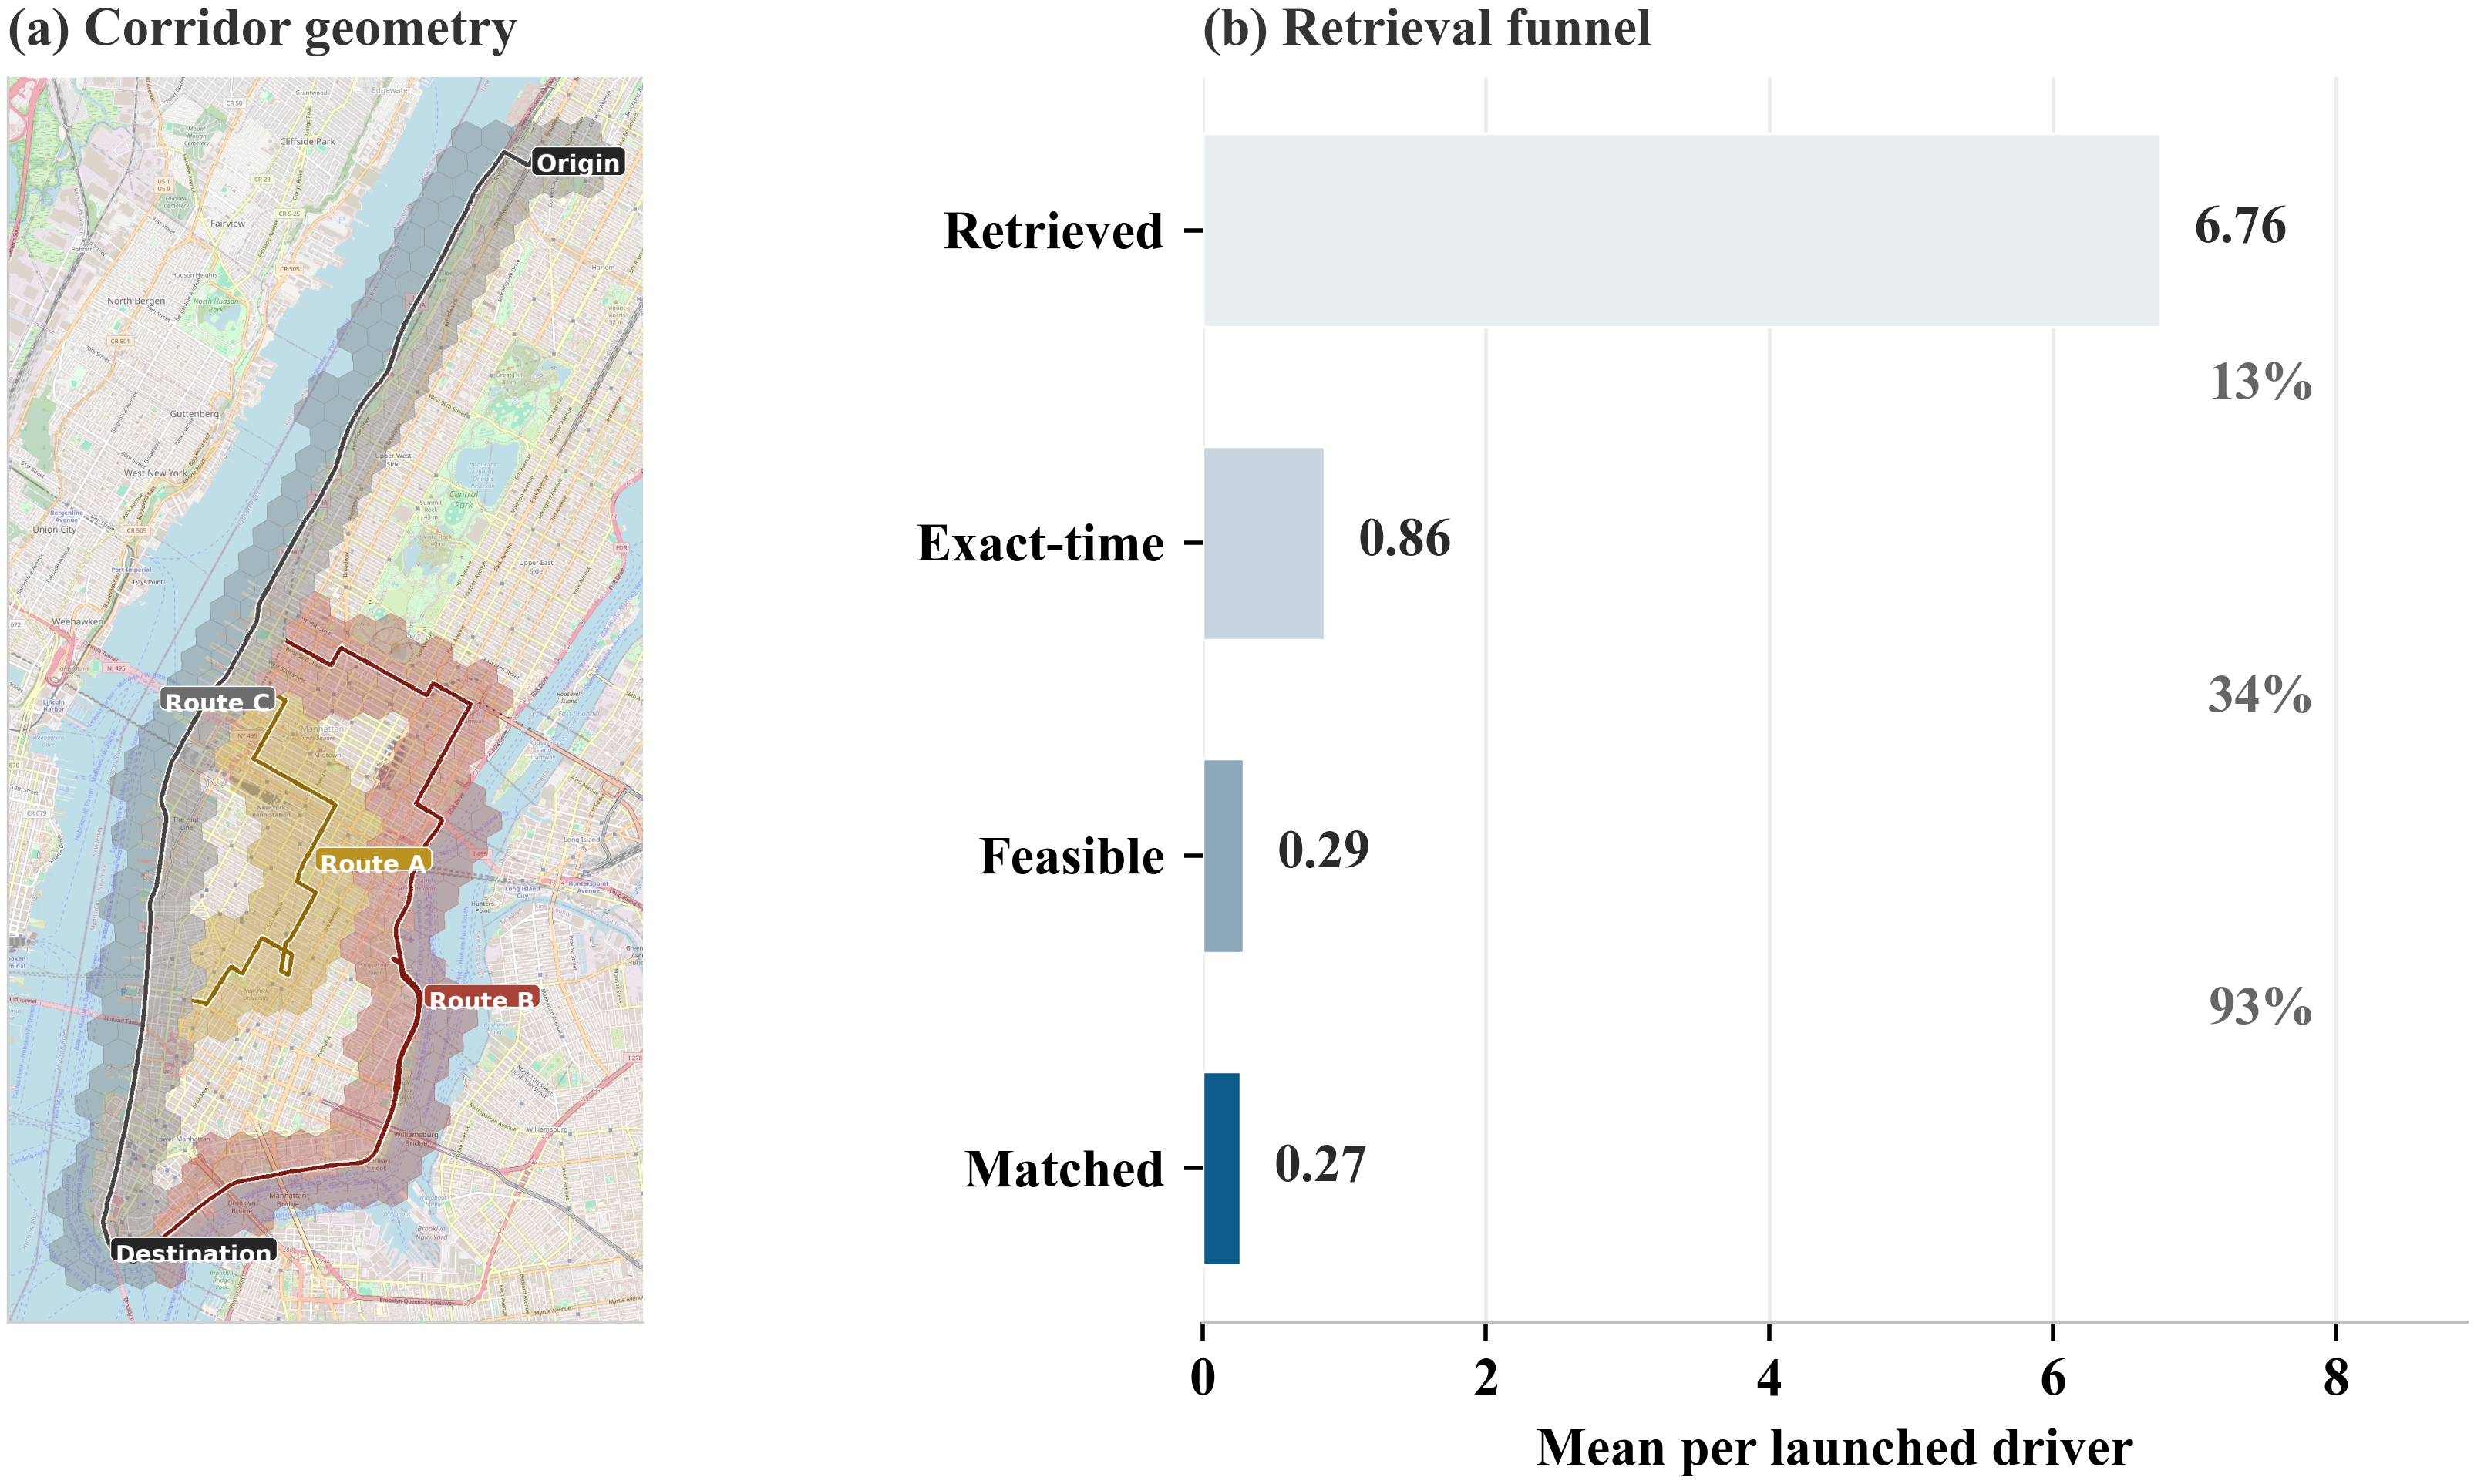
\includegraphics[width=\textwidth]{figures/paper_fig2_matching_ball_mechanism.png}
\caption{Matching-ball mechanism. Panel (a) depicts the \emph{spatial} layer of matching-ball retrieval: three illustrative OSRM alternatives are shown as route-specific H3 corridors with one-ring expansion at H3 resolution 9 (\(k=1\)); Route A is yellow, Route B is red, and Route C is gray, with origin and destination markers shown explicitly on the map. The map alone does not encode the time window or feasibility rules; those are applied afterward. Panel (b) shows the Yellow 10\% stress-test dispatch funnel for the warm-up policy: retrieved corridor candidates average 6.76 per launched driver, 0.86 remain dispatch-available after exact-time filtering, 0.29 survive detour/seat feasibility, and 0.27 are finally matched riders.}
\label{fig:matching_ball}
\end{figure*}

Figure~\ref{fig:matching_ball} shows the effect of exact timing. Retrieved corridor candidates are numerous, but only a small subset remain simultaneously open in the request pool and exact-window compatible at the driver's actual departure time. In the Yellow 10\% stress-test scenario, only about 13\% of retrieved corridor candidates survive that dispatch-availability filter, and only a smaller subset survive detour and seat checks. Matching-ball retrieval is therefore both route-aware and timing-aware.

The route alternatives also expose meaningfully different candidate pools. On 100 cached April Yellow drivers with multiple route alternatives, mean route-cell Jaccard overlap across alternatives is 0.31, mean exact-window candidate overlap is 0.35, and mean feasible-candidate overlap falls to 0.26. The best available alternative improves realized route-set profit over the default route by \(\$4.75\) on average and \(\$0.20\) at the median, showing a heavy-tailed but operationally real route-choice opportunity. Table~\ref{tab:eligibility_ablation} further shows why the paper keeps the stricter pickup-and-drop-off rule: pickup-only and drop-off-only retrieval return roughly five times as many exact-window riders, but that looser exposure would no longer represent a route-feasible pooled trip.

\begin{table}[!t]
\caption{Eligibility-rule ablation on cached April Yellow route alternatives. Only the pickup-and-drop-off rule is passed through detour and seat feasibility.}
\label{tab:eligibility_ablation}
\centering
\scriptsize
\setlength{\tabcolsep}{3.5pt}
\begin{tabular}{|l|r|r|}
\hline
Eligibility rule & Exact-time candidates & Detour/seat feasible \\
\hline
Pickup only & 78.12 & -- \\
\hline
Drop-off only & 76.25 & -- \\
\hline
Pickup and drop-off & 13.96 & 4.32 \\
\hline
\end{tabular}
\end{table}

\subsection{Route-Ranking Policies}
Among feasible riders, seat assignment is greedy by fare with seed-controlled tie-breaking. Let \(\Gamma(\mathcal{U}_r^{\mathrm{feas}},s_d)\) denote that greedy seat-assignment operator, so that \(M_r=\Gamma(\mathcal{U}_r^{\mathrm{feas}},s_d)\). For route \(r\), realized scenario profit is
\[
g(d,r)= \alpha \sum_{u\in M_r}f_u - c\cdot \ell_r,
\]
where \(f_u\) is rider fare, \(\alpha\) is platform share, \(c\) is cost per mile, and \(\ell_r\) is route distance in miles. Policies differ only in the route score \(s_\phi(d,r)\) used to select
\[
r_d^\phi=\arg\max_{r\in\mathcal{R}_d}s_\phi(d,r).
\]

\begin{table}[!t]
\caption{Route-selection policies and score definitions.}
\label{tab:policy_definitions}
\centering
\footnotesize
\begin{tabularx}{\columnwidth}{|L{0.24\columnwidth}|Y|L{0.18\columnwidth}|}
\hline
Policy & Score definition \(s_\phi(d,r)\) & Deployable online? \\
\hline
Cold-start & Indicator for the first OSRM route & Yes \\
\hline
Random & Uniform draw over \(\mathcal{R}_d\) & Yes \\
\hline
Heuristic count & \(|\mathcal{U}_r^{\mathrm{cand}}|\) & Yes \\
\hline
Heuristic fare density & Corridor fare density summary & Yes \\
\hline
Heuristic feasible count & \(|\mathcal{U}_r^{\mathrm{feas}}|\) & Yes \\
\hline
Heuristic profit proxy & Hand-built non-ML value proxy & Yes \\
\hline
ML warm-up & Predicted scenario profit \(\hat g(d,r)\) & Yes \\
\hline
Oracle (route set) & Realized scenario profit \(g(d,r)\) & No \\
\hline
\end{tabularx}
\end{table}

Table~\ref{tab:policy_definitions} lists all route-selection policies. To avoid choosing a heuristic only after seeing the April test set, a March 2015 validation probe over cached Yellow route alternatives selects fare-density as the deployable non-ML rule. On the April primary dispatch test, feasible-rider count performs better than the validation-selected rule; we therefore report feasible-rider count as a conservative upper heuristic benchmark while retaining the validation-selected fare-density comparison in the text and reproducibility outputs.

Because fare-greedy seat fill is another possible source of bias, we compared it with an exhaustive small-batch assignment over the same feasible rider sets on 200 cached route cases. Greedy assignment is equal to the exhaustive optimum in 93\% of cases; when averaged over all route cases, exhaustive assignment raises rider revenue from \(\$11.90\) to \(\$12.42\), a \(\$0.51\) mean revenue gap before route-distance cost. We therefore keep the greedy rule for low-latency dispatch, but treat it as a conservative implementation choice rather than an optimal seating solver.

\section{Rolling-Horizon Dispatch Design}
The main paper contribution is not only route ranking in isolation, but route ranking embedded inside a shared rider pool. We therefore add a rolling-horizon dispatch simulator with 60-second batching. Let \(\mathcal{U}_b\) denote the open request pool at batch \(b\). Drivers are scored route-by-route against \(\mathcal{U}_b\), and each policy produces a provisional score
\[
\omega_d^\phi=s_\phi\!\left(d,r_d^\phi\right),
\]
where \(r_d^\phi\) is the provisional best route for driver \(d\) under policy \(\phi\). Active drivers in the batch are processed in descending \(\omega_d^\phi\), with deterministic fallback to departure time.

When a driver is finalized, the corresponding matched riders are removed from the pool:
\[
\mathcal{U}_b^{(j+1)}=\mathcal{U}_b^{(j)}\setminus M_{r_{d_j}^{\phi}},
\]
where \(d_j\) is the \(j\)-th driver in batch order. The next driver is then re-evaluated once against \(\mathcal{U}_b^{(j+1)}\). This one-step conflict recomputation is sufficient to enforce rider exclusivity while keeping the simulation low latency. Algorithm~\ref{alg:dispatch} formalizes the full batch loop.

\begin{algorithm}[!t]
\caption{Route-aware retrieval and scoring for one driver}
\label{alg:route_scoring}
\footnotesize
\begin{algorithmic}[1]
\Require Driver \(d\), policy \(\phi\), route cache / OSRM client
\Statex \hspace{\algorithmicindent} Open request pool \(\mathcal{U}_b\)
\State Retrieve \(\mathcal{R}_d\) from cache; on miss request up to \(K=3\) OSRM alternatives
\If{\(\mathcal{R}_d=\emptyset\)}
    \State \Return no-launch / cache-miss failure case
\EndIf
\ForAll{\(r \in \mathcal{R}_d\)}
    \State Build corridor \(C_r\) from the densified route spine
    \State Retrieve \(\mathcal{U}_r^{\mathrm{cand}}\) from the H3/time index
    \State Filter to \(\mathcal{U}_r^{\mathrm{feas}}\) using
    \Statex \hspace{\algorithmicindent} exact time, directionality, detour, and seats
    \State Intersect feasible riders with currently open pool \(\mathcal{U}_b\)
    \State Compute \(M_r=\Gamma(\mathcal{U}_r^{\mathrm{feas}},s_d)\) by greedy seat assignment
    \State Compute realized route value \(g(d,r)\) and policy score \(s_\phi(d,r)\)
\EndFor
\State Break score ties by smaller route index, then deterministic seed order
\State \Return \(r_d^\phi=\arg\max_{r \in \mathcal{R}_d}s_\phi(d,r)\)
\end{algorithmic}
\end{algorithm}

\begin{algorithm}[!t]
\caption{Rolling-horizon dispatch with one-step conflict recomputation}
\label{alg:dispatch}
\footnotesize
\begin{algorithmic}[1]
\Require Batched driver stream, batched rider stream
\Statex \hspace{\algorithmicindent} Policy \(\phi\)
\State Initialize open request pool \(\mathcal{U}_b \gets \emptyset\)
\For{each dispatch batch \(b\)}
    \State Add newly observed riders to \(\mathcal{U}_b\)
    \State Remove riders whose exact request window has elapsed
    \State Activate drivers whose departure times fall inside batch \(b\)
    \ForAll{active drivers \(d\)}
        \State Compute provisional route \(r_d^\phi\) using Algorithm~\ref{alg:route_scoring}
        \State Set ordering score \(\omega_d^\phi=s_\phi(d,r_d^\phi)\)
    \EndFor
    \State Sort active drivers by descending \(\omega_d^\phi\), breaking ties by departure time
    \ForAll{sorted drivers \(d_j\)}
        \State Recompute route scores once against the current pool \(\mathcal{U}_b^{(j)}\)
        \State Finalize \(r_{d_j}^{\phi}\) and matched set \(M_{r_{d_j}^{\phi}}\)
        \State Update \(\mathcal{U}_b^{(j+1)} \gets \mathcal{U}_b^{(j)} \setminus M_{r_{d_j}^{\phi}}\)
        \State Remove launched driver \(d_j\) from the active set
    \EndFor
\EndFor
\end{algorithmic}
\end{algorithm}

This is still a dispatch approximation. It does not reposition vehicles, optimize global assignment over long horizons, or keep launched drivers active after commitment. Once a driver launches on a route, that driver exits the batch system. The simulator should therefore be read as a low-latency route-choice layer embedded in a rolling shared-request environment, not as a full production dispatch platform.

\section{Experimental Design}
\subsection{System-Level Dispatch}
The dispatch experiments use 1000 April 2015 Yellow test drivers and five seeds. Repeat-run summaries are aggregated at the seed level before reporting intervals across retained-sample seeds, although many of those intervals collapse visually because the simulator is nearly deterministic once the retained rider sample is fixed. These intervals should therefore be read as repeat-run dispersion under the retained-sample protocol rather than as broad inferential uncertainty. The headline dispatch assumptions are:
\begin{itemize}
    \item domain = Yellow,
    \item batch cadence = 60 seconds,
    \item retained-sample density = 10\%,
    \item exact request window = 5 minutes,
    \item max detour = 4 minutes.
\end{itemize}

Additional dispatch sweeps vary density \(\{100,25,10\}\), request window \(\{2,5,10\}\) minutes, and detour \(\{2,4,6\}\) minutes. The public second-domain experiment repeats the 10\% stress-test dispatch scenario and density sweep on Green using the same January--February 2015 train, March 2015 validation, April 2015 test structure.

\subsection{Controlled Single-Driver Analysis}
The isolated-driver paired analysis uses 5{,}000 April Yellow test drivers and five seeds. Each strategy sees the same driver, rider snapshot, route set, and random seed; only the route-selection rule changes. This larger controlled study is retained because it isolates route-ranking effects without driver competition.

\subsection{Model Development and Metrics}
Yellow model development uses January--February 2015 for training and March 2015 for validation and selection; the final deployed Yellow model is retrained on January--March before April evaluation. The same temporal pattern is used for Green. The tuned model uses 38 features that exclude realized matching outputs, spanning geometry, temporal context, spatial demand, and landmark/cell context.

Table~\ref{tab:feature_dictionary} lists the feature families. All features are available at route-scoring time: route geometry comes from OSRM alternatives, online corridor demand comes from the currently open request pool, temporal features come from the driver departure timestamp, and historical H3/cell summaries are precomputed from earlier training months only. No feature uses realized April matching outcomes or the route's eventual policy selection.

\begin{table*}[!t]
\caption{Feature dictionary used by the route-value scorer. The reproducibility package writes the same dictionary with source, availability, aggregation window, and leakage status.}
\label{tab:feature_dictionary}
\centering
\scriptsize
\begin{tabularx}{\textwidth}{|L{0.16\textwidth}|L{0.65\textwidth}|Y|}
\hline
Family & Features & Availability / leakage status \\
\hline
Route geometry & \texttt{route\_distance\_m}, \texttt{route\_duration\_s}, \texttt{corridor\_cell\_count}, \texttt{route\_sinuosity}, \texttt{route\_avg\_speed\_ms}, \texttt{bearing\_sin}, \texttt{bearing\_cos}, \texttt{straight\_line\_dist\_m} & Computed from driver OD and OSRM route before route choice; no realized matching output. \\
\hline
Temporal context & \texttt{hour\_of\_day}, \texttt{day\_of\_week}, \texttt{is\_weekend}, \texttt{day\_of\_month}, \texttt{time\_bin\_15min}, \texttt{hour\_sin}, \texttt{hour\_cos} & Driver departure-time features available at dispatch time. \\
\hline
Online corridor demand & \texttt{corridor\_rider\_count}, \texttt{corridor\_demand\_density}, \texttt{mean\_rider\_fare}, \texttt{corridor\_fare\_density} & Computed from exact-window open candidates before assignment; not from final matched riders. \\
\hline
Historical spatial demand & \texttt{corridor\_hist\_pickups}, \texttt{corridor\_hist\_dropoffs}, \texttt{corridor\_hist\_pickup\_density}, \texttt{corridor\_hist\_dropoff\_density}, \texttt{corridor\_hist\_mean\_fare}, \texttt{corridor\_hist\_fare\_density}, \texttt{origin\_cell\_pickups}, \texttt{origin\_cell\_mean\_fare}, \texttt{dest\_cell\_dropoffs} & Precomputed from training/history months before evaluation. \\
\hline
Landmark/cell context & \texttt{origin\_landmark\_dist\_km}, \texttt{dest\_landmark\_dist\_km}, \texttt{origin\_jfk\_km}, \texttt{origin\_lga\_km}, \texttt{origin\_penn\_km}, \texttt{origin\_times\_sq\_km}, \texttt{dest\_jfk\_km}, \texttt{dest\_lga\_km}, \texttt{dest\_penn\_km}, \texttt{dest\_times\_sq\_km} & Static distances from driver OD to fixed NYC references; no outcome leakage. \\
\hline
\end{tabularx}
\end{table*}

For a policy \(\phi\), the main reported system metrics are
\begin{equation}
\begin{aligned}
\bar g_\phi &= \frac{1}{|\mathcal{D}_\phi^{\mathrm{launch}}|}
\sum_{d \in \mathcal{D}_\phi^{\mathrm{launch}}} g(d,r_d^\phi),\\
\bar m_\phi &= \frac{1}{|\mathcal{D}_\phi^{\mathrm{launch}}|}
\sum_{d \in \mathcal{D}_\phi^{\mathrm{launch}}} |M_{r_d^\phi}|,
\end{aligned}
\end{equation}
that is, scenario profit per launched driver and matched riders per launched driver. Because \(\bar g_\phi\) is negative in the sparse regimes, the main presentation in the Results section emphasizes \emph{operating loss} and \emph{loss reduction} relative to cold-start rather than absolute profit creation.

We report:
\begin{itemize}
    \item \textbf{System metrics:} scenario profit per launched driver, operating loss per launched driver, rider service rate, mean wait, matched riders per driver, seat occupancy, and dispatch runtime.
    \item \textbf{Model metrics:} \(R^2\), RMSE, MAE, and route rank-1 accuracy.
    \item \textbf{Paired gaps:} mean driver-level differences, bootstrap confidence intervals, and win/tie/loss rates in the isolated-driver study.
\end{itemize}

\section{Results}
\subsection{Primary Yellow Sparse Dispatch}
Tables~\ref{tab:dispatch_primary} and \ref{tab:dispatch_delta} report the main dispatch results. Under 60-second batching, a 5-minute exact request window, and 10\% retained-sample density, route-aware policies reduce loss relative to cold-start even in a thin rider market. ML warm-up gives the best realizable policy, although the margin over the strongest heuristic remains modest and comes from route-value tradeoffs rather than from serving strictly more riders.

The March validation probe selects the fare-density heuristic, which records \(\$7.37\) loss per launched driver on April. The feasible-count rule is stronger on April at \(\$7.30\) loss per driver, so the table's ``Best heuristic'' row uses feasible-count as a harder conservative benchmark rather than the easier validation-selected comparator.

\begin{table}[!t]
\caption{Primary Yellow sparse dispatch outcomes: 60-second batches, 5-minute exact request window, 10\% retained-sample density, 4-minute detour, 1000 drivers, five seeds.}
\label{tab:dispatch_primary}
\centering
\scriptsize
\setlength{\tabcolsep}{2.6pt}
\begin{tabular}{|l|r|r|r|r|}
\hline
Policy & Loss/driver (\$) & Loss reduction & Matched/driver & Wait (min) \\
\hline
Cold-start & 8.08 & --- & 0.16 & 2.51 \\
\hline
Best heuristic & 7.30 & 0.78 & 0.29 & 2.52 \\
\hline
ML warm-up & \textbf{7.15} & \textbf{0.93} & 0.27 & 2.56 \\
\hline
Oracle (route set) & 7.02 & 1.06 & 0.29 & 2.54 \\
\hline
\end{tabular}
\end{table}

\begin{table}[!t]
\caption{Comparative interpretation and seed-level dispatch policy-gap summary. Intervals collapse to the same value under the retained-sample seeds, so these are point estimates rather than broad inferential intervals.}
\label{tab:dispatch_delta}
\label{tab:dispatch_policy_gap}
\centering
\footnotesize
\begin{tabularx}{\columnwidth}{|Y|r|r|}
\hline
Comparison & Delta (\$/driver) & Relative loss reduction \\
\hline
Yellow best heuristic vs.\ cold-start & +0.78 & 9.7\% \\
\hline
Yellow ML warm-up vs.\ cold-start & +0.93 & 11.5\% \\
\hline
Yellow oracle vs.\ cold-start & +1.06 & 13.1\% \\
\hline
Yellow ML warm-up vs.\ best heuristic & +0.15 & 1.9\% \\
\hline
Yellow ML warm-up vs.\ validation-selected heuristic & +0.22 & 2.7\% \\
\hline
Green ML warm-up vs.\ cold-start & +0.39 & 5.1\% \\
\hline
Green ML warm-up vs.\ best heuristic & +0.27 & 3.6\% \\
\hline
\end{tabularx}
\end{table}

The route-aware layer reduces operating loss relative to cold-start by \(\$0.93\) per launched driver, or about 11.5\%, in the sparse regime. The learned ranker adds a smaller increment: \(\$0.15\) per driver over the conservative April-best heuristic and \(\$0.22\) over the March validation-selected heuristic, while the strongest heuristic matches slightly more riders. Table~\ref{tab:dispatch_policy_gap} records these seed-level gaps for both Yellow and Green. Because the retained rider samples make the dispatch runs nearly deterministic, the gap intervals collapse to the reported point estimates; the result should be read as a repeat-run policy comparison, not as a population-level uncertainty interval. The reproducibility materials include a dispatch CI-width audit over the headline and density-sweep metrics; all checked seed-level dispatch intervals collapse under this retained-sample protocol.

\subsection{Dispatch Density Response}
Figure~\ref{fig:dispatch_density} places the 10\% sparse headline result inside the full Yellow dispatch density sweep, plotting \emph{savings over cold-start} so the policy ordering is legible at every density level. At 10\% retained-sample density, the strongest heuristic saves \(\$0.78\) per launched driver relative to cold-start, ML warm-up saves \(\$0.93\), and the within-route-set oracle saves \(\$1.06\). At 25\%, the corresponding savings are \(\$1.24\), \(\$1.39\), and \(\$1.57\). At the full 100\% retained-sample benchmark, they are \(\$2.20\), \(\$2.31\), and \(\$2.75\). Savings increase as the rider pool densifies. The simulator is near-deterministic across seeds at fixed density; repeat-run variation is smaller than the marker size.

As a geometric sanity baseline, we also evaluate a 1 km path-buffer policy on 1000 Yellow test drivers and five seeds using the same exact-time and detour rules. The run uses live-or-cached OSRM routes and therefore matches the scale of the primary dispatch headline. The comparator improves upon cold-start but remains weaker than matching-ball retrieval. In dispatch at 10\%, the path-buffer policy reduces loss from \(\$8.25\) to \(\$8.07\), whereas the strongest matching-ball heuristic reaches \(\$7.30\). In the controlled single-driver study, the same path-buffer policy improves 25\% loss from \(\$4.95\) to \(\$4.40\) and 10\% loss from \(\$7.20\) to \(\$6.92\), but still trails the corresponding best matching-ball heuristic at \(\$3.53\) and \(\$6.28\). This check indicates that the H3 corridor construction is not merely reproducing what a simple geometric buffer already captures.

Two additional cached-subset dispatch diagnostics use 100 multi-route April Yellow drivers at 10\% retained density. A greedy nearest-route dispatcher, which chooses the route with the lowest mean feasible rider detour before enforcing rider exclusivity, obtains \(-\$7.61\) per driver and 0.28 matched riders per driver. A single-rider batch bipartite assignment baseline, which globally matches drivers to at most one feasible rider by maximum edge weight, obtains \(-\$8.59\) per driver and 0.05 matched riders per driver. These diagnostics are not production RTV solvers, but they provide assignment-style comparisons alongside the route-count heuristics.

\begin{figure*}[!t]
\centering
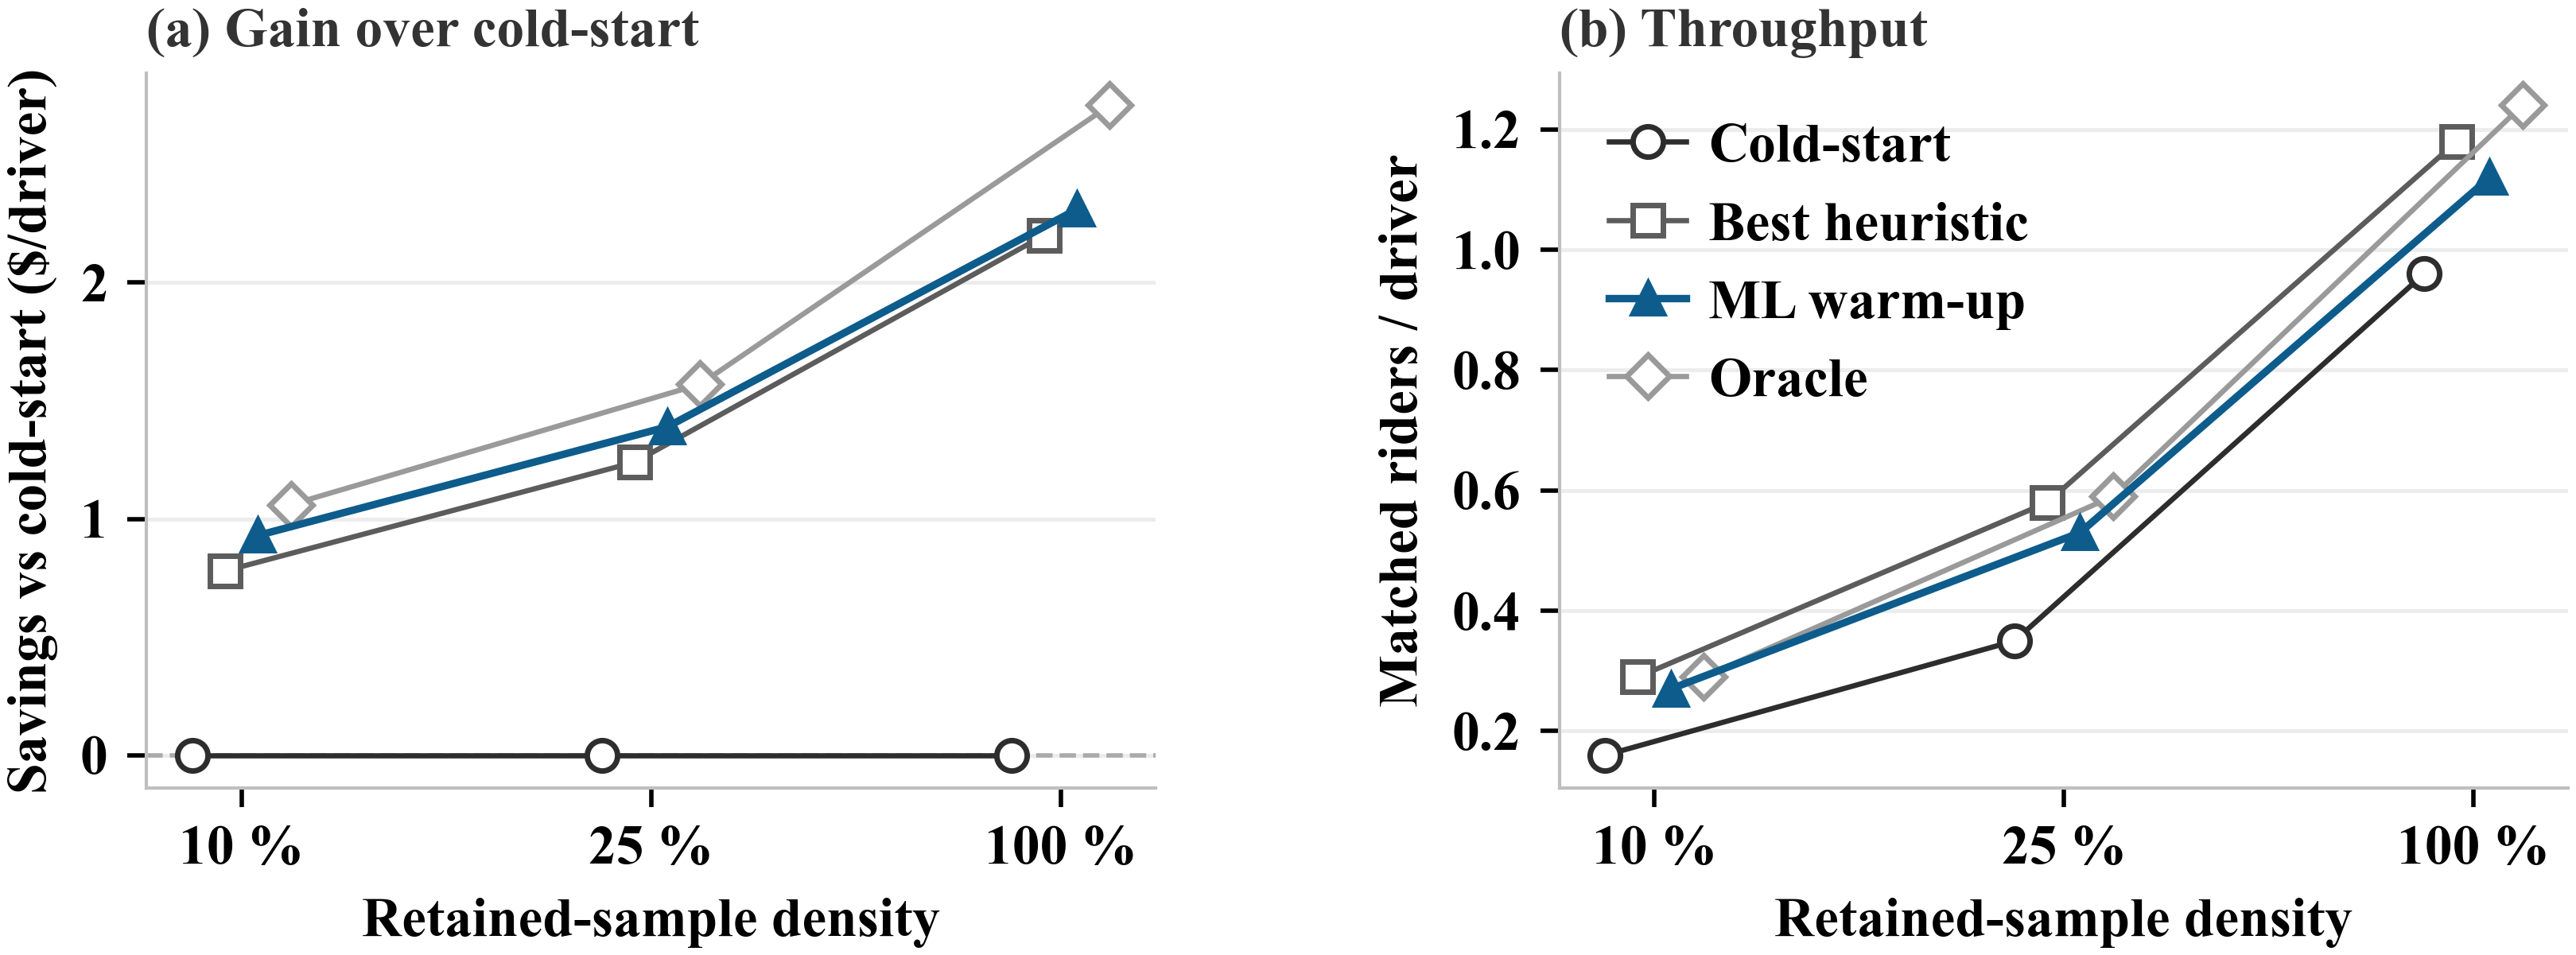
\includegraphics[width=\textwidth]{figures/paper_fig3_dispatch_density.png}
\caption{Dispatch density response under 60-second batches and a 5-minute exact request window. \emph{(a)} Savings over cold-start per launched driver (cold-start = \$0 reference line); plotting the \emph{gain} rather than the absolute loss spreads the policy lines and makes the ordering readable at every density. \emph{(b)} Matched riders per launched driver. The best heuristic leads ML warm-up in throughput at every density because it directly maximises compatible rider count (\texttt{heuristic\_feasible\_count}), whereas ML warm-up optimises route profit; the two objectives diverge slightly under sparse supply. The x-axis runs sparse (10\%) to dense (100\%), where 100\% refers to the full pre-sampled 25\% rider pool. The simulator is near-deterministic across seeds at fixed density; repeat-run variation is smaller than the marker size.}
\label{fig:dispatch_density}
\end{figure*}

\subsection{Same-City Service-Type Robustness}
Table~\ref{tab:domain_transfer} reports the same-city Yellow--Green comparison for the harsher 10\% stress-test regime. Green reproduces the same qualitative hierarchy as Yellow: cold-start is worst, warm-up is better, and the oracle within the route set remains the upper bound. The Green stress test is slightly less negative overall, and its wait times are lower. Because both public domains are NYC taxi services, this result should be read as a service-type comparison under similar telemetry rather than as an external-city validation.

\begin{table}[!t]
\caption{Stress-test dispatch scenario across NYC public service types. Yellow and Green both use 60-second batching, a 5-minute exact request window, 10\% retained-sample density, 4-minute detour, 1000 drivers, and five seeds. Comparative deltas are interpreted relative to the domain-specific cold-start baseline.}
\label{tab:domain_transfer}
\centering
\scriptsize
\setlength{\tabcolsep}{2.4pt}
\begin{tabular}{|l|r|r|r|r|}
\hline
Policy & Yellow loss & Green loss & Yellow wait & Green wait \\
\hline
Cold-start & 8.08 & 7.66 & 2.51 & 1.87 \\
\hline
Best heuristic & 7.30 & 7.54 & 2.52 & 2.14 \\
\hline
ML warm-up & \textbf{7.15} & \textbf{7.27} & 2.56 & 2.07 \\
\hline
Oracle (route set) & 7.02 & 7.25 & 2.54 & 2.05 \\
\hline
\end{tabular}
\end{table}

The warm-up edge over the strongest heuristic is \(\$0.15\) per launched driver in Yellow and \(\$0.27\) in Green. That is still a modest margin, but it persists in the same-city service-type shift. The result supports a narrow claim: route-aware retrieval plus exact timing help dispatch, and ML is a competitive route-ranker rather than a source of large gains under this stress test.

\subsection{Controlled Single-Driver Mechanism}
The dispatch results answer the system question, but they do not isolate route-ranking effects. Figures~\ref{fig:single_driver_gain_comp} and \ref{fig:single_driver_residual} therefore compare the larger single-driver paired study against the dispatch layer under the same exact-timing assumptions. In the controlled experiment, the 10\% sparse regime moves from \(\$7.40\) loss under cold-start to \(\$6.17\) under ML warm-up, while the strongest heuristic reaches \(\$6.28\) and the within-route-set oracle reaches \(\$5.95\). At 25\%, the corresponding losses are \(\$5.26\), \(\$3.53\), \(\$3.42\), and \(\$3.08\). Figure~\ref{fig:single_driver_gain_comp} shows that, in both dispatch and isolated evaluation, most of the route-aware gain is already recovered by the strongest heuristic, with ML adding a smaller residual lift and the oracle retaining limited headroom. Figure~\ref{fig:single_driver_residual} then compares the warm-up-vs-strongest-heuristic gap directly across densities in both evaluation layers. The main result is not that competition always collapses the ML edge; it is that the ML contribution remains secondary to heuristic recovery in both layers and never becomes the dominant source of route-aware gain.

In the single-driver study, the 10\% warm-up-versus-strongest-heuristic gap is \(\$0.11\) with bootstrap interval \([\$0.07,\$0.16]\); at 25\%, the corresponding gap is \(\$0.10\) with interval \([\$0.05,\$0.16]\). These paired gaps confirm that the learned scorer retains signal beyond the heuristic, but only as a residual layer on top of route-aware retrieval.

\begin{figure}[!t]
\centering
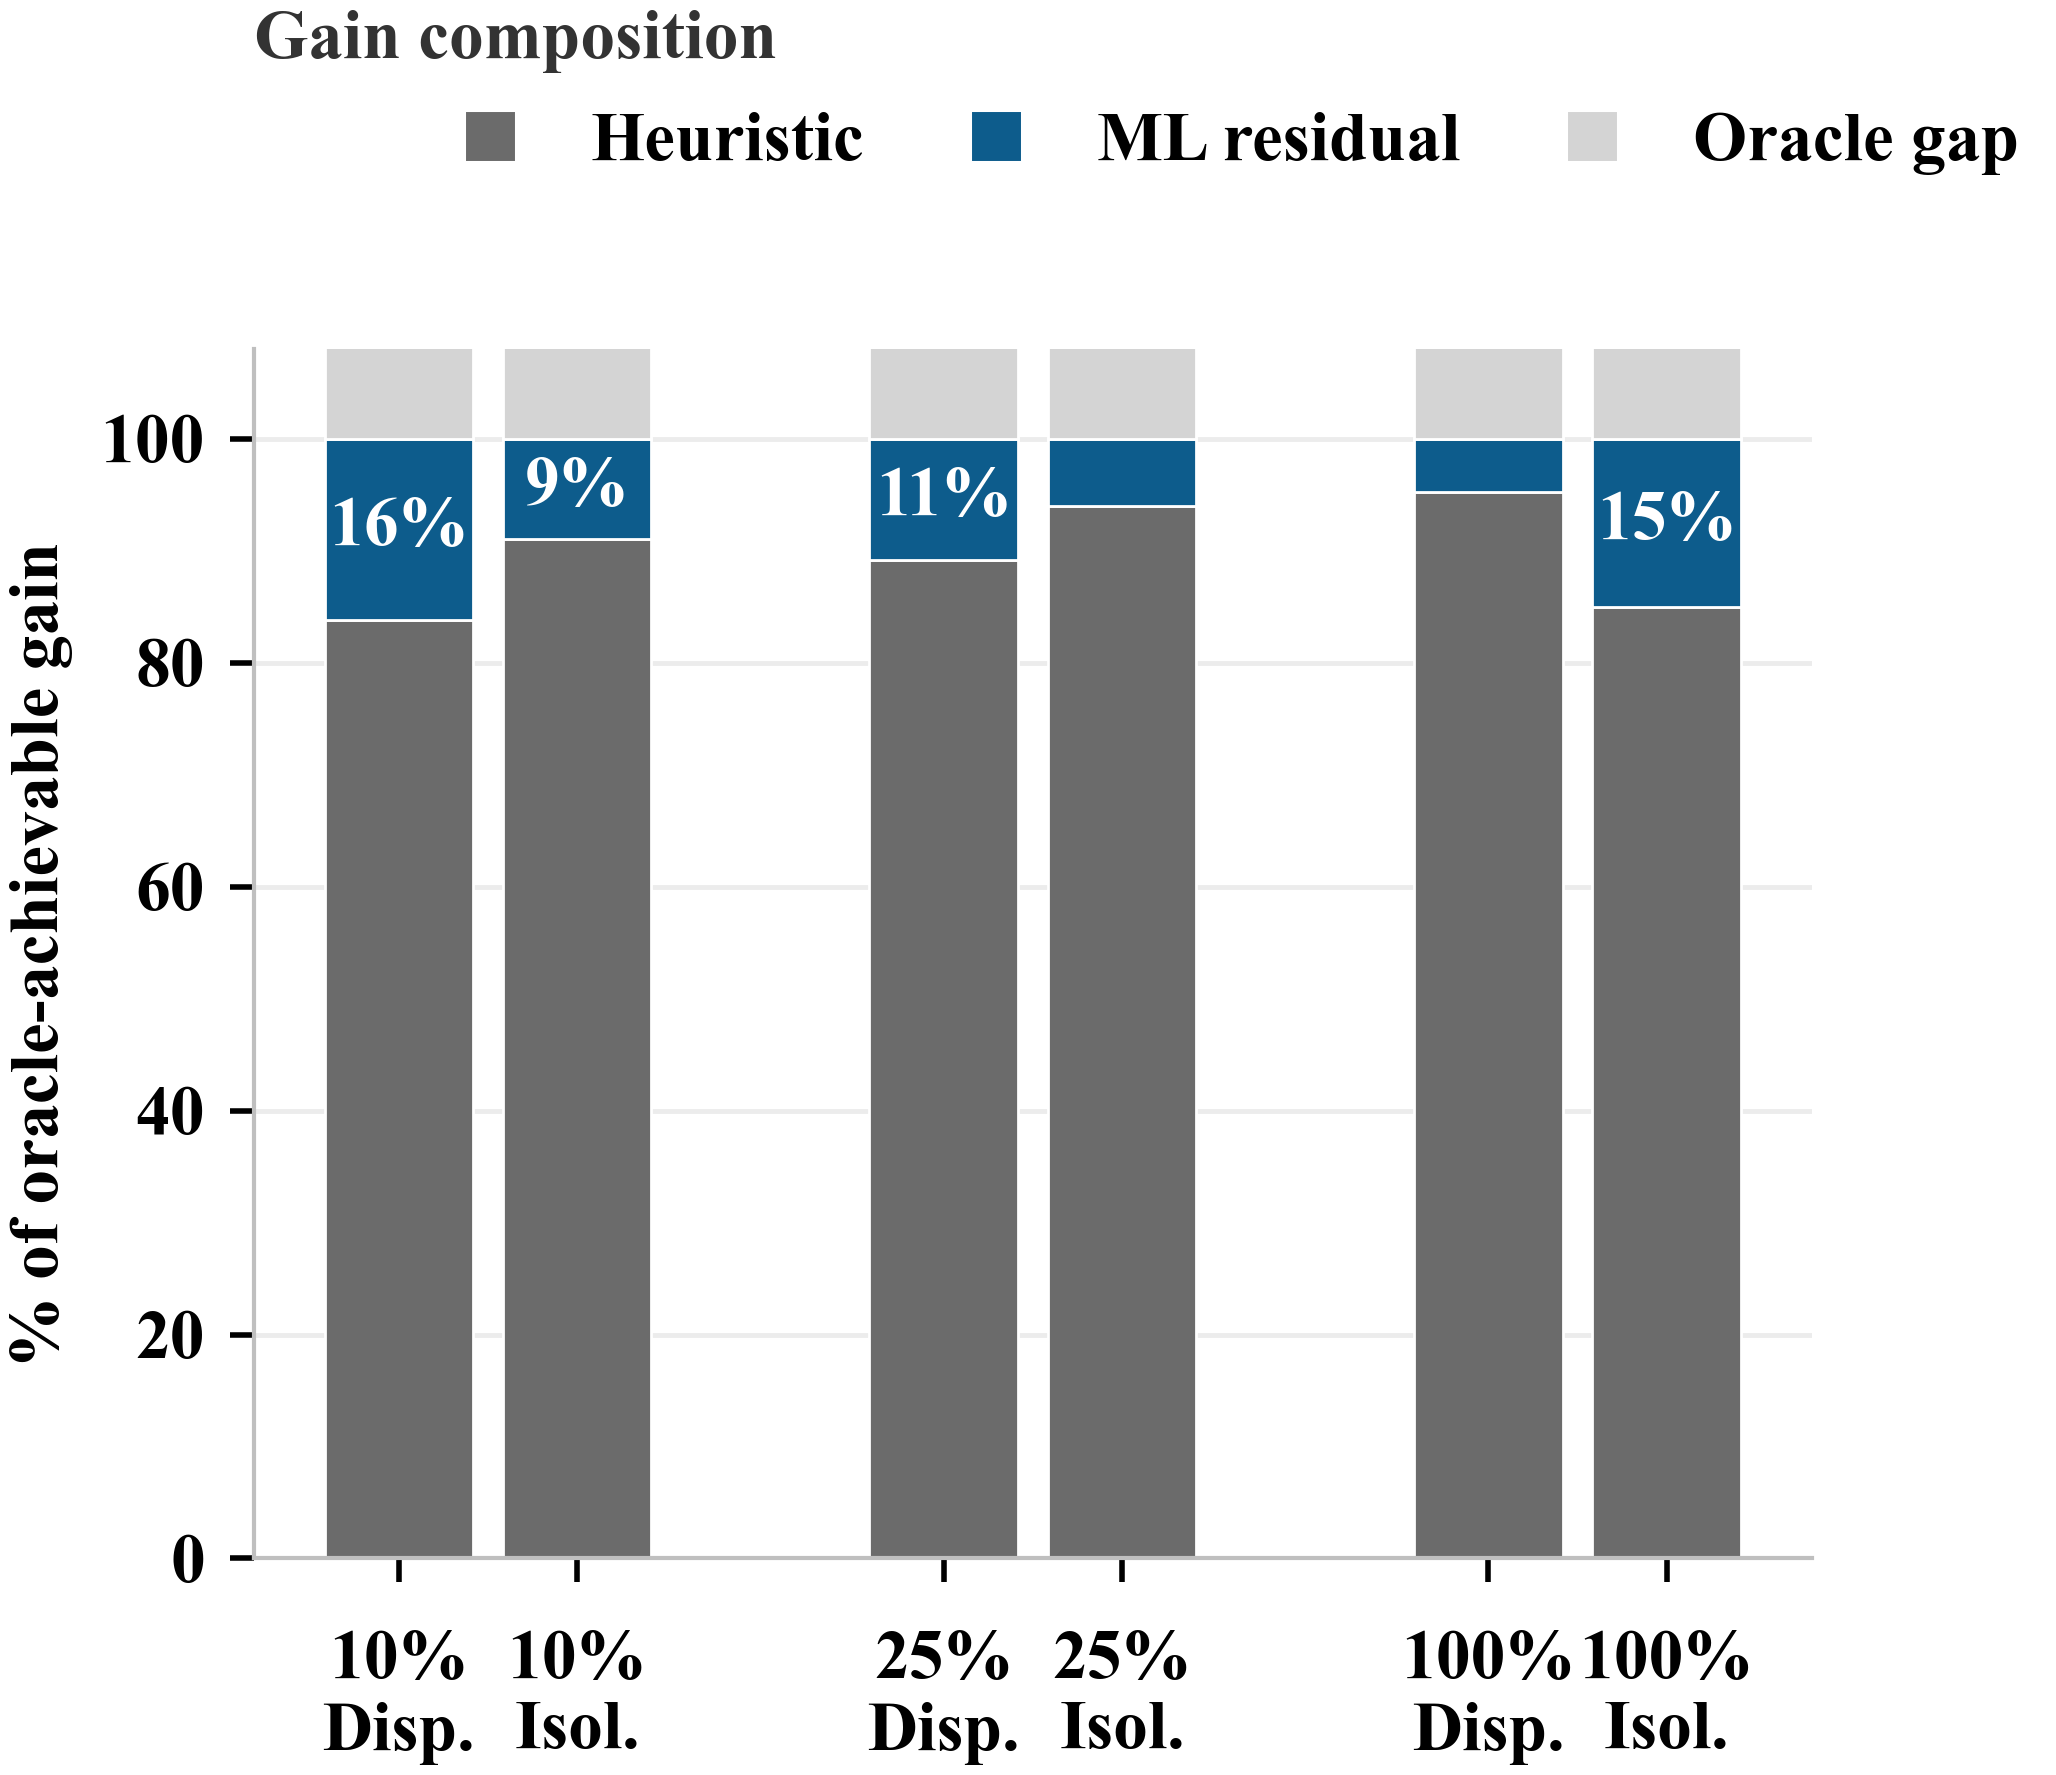
\includegraphics[width=\linewidth]{figures/paper_fig5a_gain_composition.png}
\caption{Route-aware gain decomposition across evaluation layers. 100\%-stacked bars show the composition of oracle-achievable gain at each density and evaluation layer (Disp.\ = rolling dispatch; Isol.\ = controlled single-driver study). Heuristic recovery accounts for 83--95\% of achievable gain; ML residual adds 5--16\%; remaining oracle headroom is small.}
\label{fig:single_driver_gain_comp}
\end{figure}

\begin{figure}[!t]
\centering
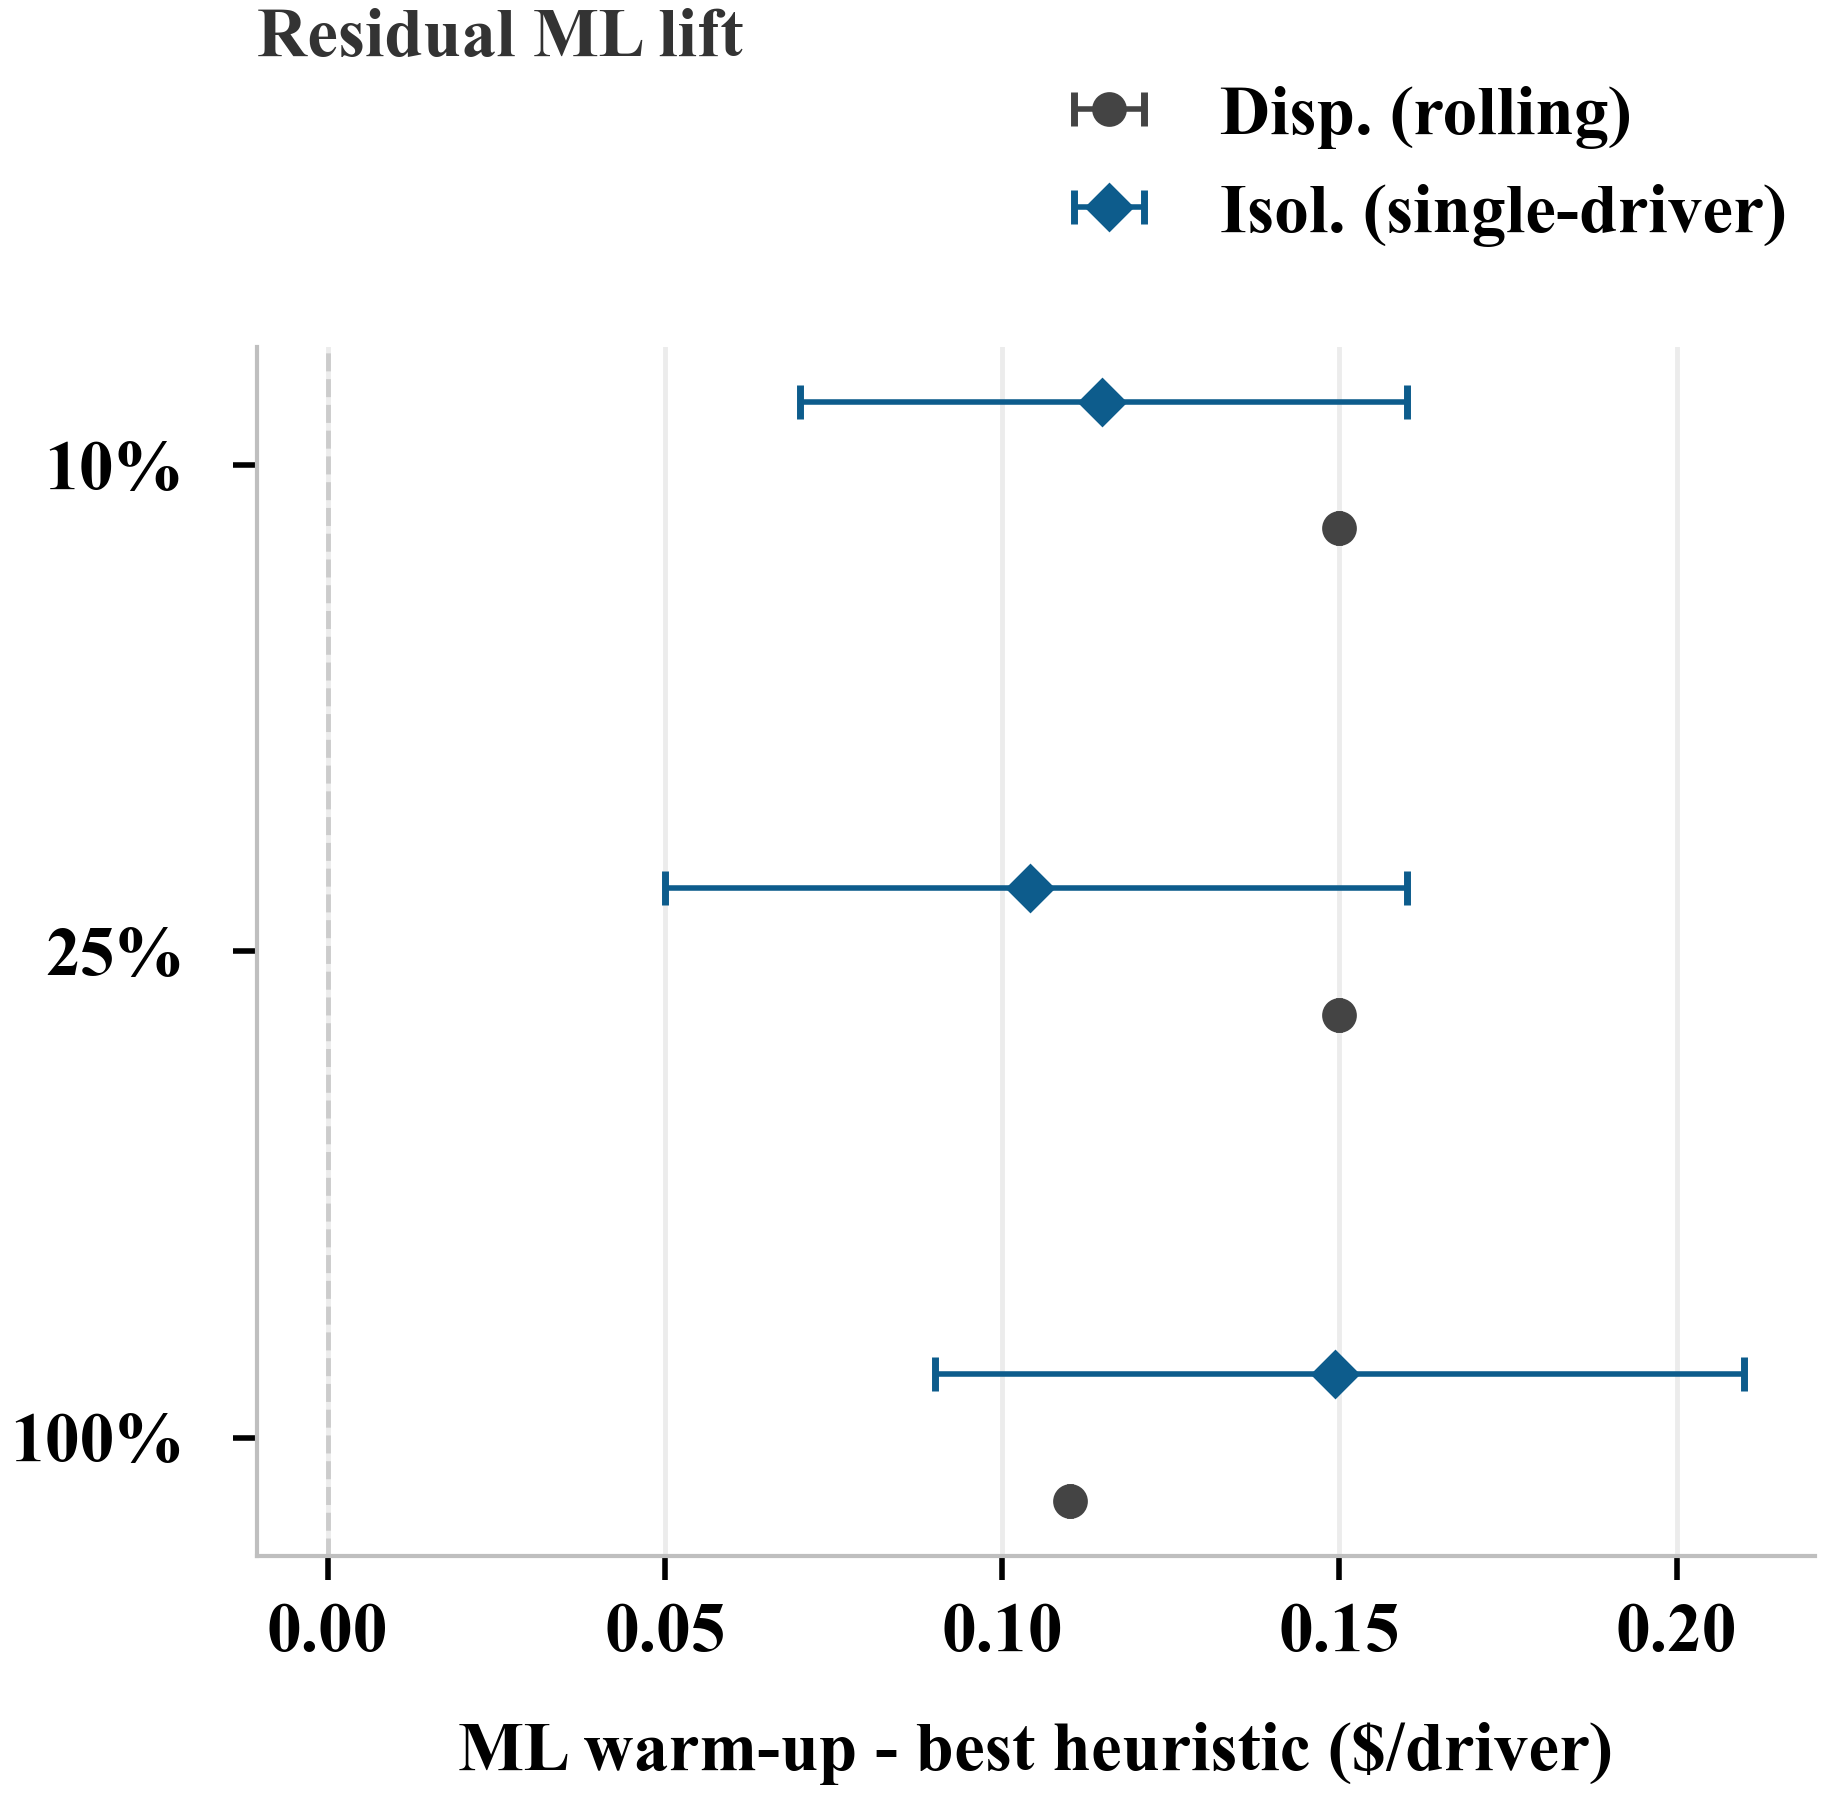
\includegraphics[width=\linewidth]{figures/paper_fig5b_residual_ml_lift.png}
\caption{Residual ML lift over the strongest heuristic. ML warm-up minus best heuristic is shown with 95\% bootstrap intervals for both evaluation layers and tested densities.}
\label{fig:single_driver_residual}
\end{figure}

The two result layers answer different questions. The single-driver study shows that the learned scorer retains a positive paired advantage over the strongest heuristic. The decomposition also shows that most of the route-aware gain is heuristic recovery. The dispatch layer then tests the residual lift under rider exclusivity and shared demand; the lift remains positive but secondary.

\subsection{Model Support}
Table~\ref{tab:model_quality} reports Yellow temporal-holdout model quality, and Figure~\ref{fig:model_support} summarizes holdout calibration for the deployed LightGBM scorer. The tuned Yellow model reaches \(R^2=0.801\), RMSE \(=\$5.85\), and 76.1\% route rank-1 accuracy. The tuned Green model reaches \(R^2=0.738\) and RMSE \(=\$2.73\). The MLP edges the Yellow holdout fit slightly with \(R^2=0.804\) and RMSE \(=\$5.81\), while LambdaRank leads rank-1 accuracy at 80.5\% but with substantially weaker absolute fit. We therefore keep tuned LightGBM because it offers the best balance of regression quality and route ranking among the models with usable score calibration. Feature-importance aggregation on the training build attributes about 89\% of total gain to spatial-demand context, 6\% to route geometry, 3\% to landmark proxies, and 2\% to coarse temporal bins, which matches the intended role of the scorer as a corridor- and demand-aware route value model rather than a single-feature shortcut.

\begin{table}[!t]
\caption{Yellow model quality on the March 2015 temporal holdout. January--February 2015 are used for training; March 2015 is used for validation and selection before final retraining on January--March for April policy evaluation.}
\label{tab:model_quality}
\centering
\scriptsize
\setlength{\tabcolsep}{2.5pt}
\begin{tabular}{|l|r|r|r|r|}
\hline
Model & \(R^2\) & RMSE & Rank-1 & Deployment role \\
\hline
Ridge (linear) & 0.692 & 6.92 & 68.1\% & Simpler baseline \\
\hline
LightGBM (baseline) & 0.786 & 6.02 & 74.2\% & Untuned tree baseline \\
\hline
LightGBM (tuned) & 0.801 & 5.85 & 76.1\% & \textbf{Selected scorer} \\
\hline
LambdaRank & 0.611 & 7.90 & \textbf{80.5\%} & Ranking-oriented, weak calibration \\
\hline
MLP (Neural Net) & \textbf{0.804} & \textbf{5.81} & 74.8\% & Slightly better fit, weaker ranking \\
\hline
\end{tabular}
\end{table}

\begin{table}[!t]
\caption{Feature-family ablation on Yellow temporal holdout.}
\label{tab:model_ablation}
\centering
\scriptsize
\setlength{\tabcolsep}{4.0pt}
\begin{tabular}{|l|r|r|}
\hline
Experiment & \(R^2\) & RMSE \\
\hline
All features & 0.801 & 5.85 \\
\hline
All minus temporal & 0.793 & 5.97 \\
\hline
All minus spatial demand & 0.721 & 6.89 \\
\hline
\end{tabular}
\end{table}

\begin{table}[!t]
\caption{Cached route-policy diagnostic by model family. This held-out diagnostic uses 42 cached multi-route April Yellow drivers at 10\% retained density and is narrower than the full rolling dispatch experiment.}
\label{tab:model_policy_diagnostic}
\centering
\scriptsize
\setlength{\tabcolsep}{3.0pt}
\begin{tabular}{|l|r|r|}
\hline
Policy scorer & Profit/driver & Rank-1 \\
\hline
Cold-start default & -7.66 & 54.8\% \\
\hline
Ridge & -6.58 & 85.7\% \\
\hline
MLP & -6.82 & 81.0\% \\
\hline
LightGBM baseline & -7.11 & 73.8\% \\
\hline
LightGBM tuned & -6.63 & 71.4\% \\
\hline
LambdaRank & -7.41 & 83.3\% \\
\hline
Oracle route set & -6.18 & 100.0\% \\
\hline
\end{tabular}
\end{table}

\begin{figure}[!t]
\centering
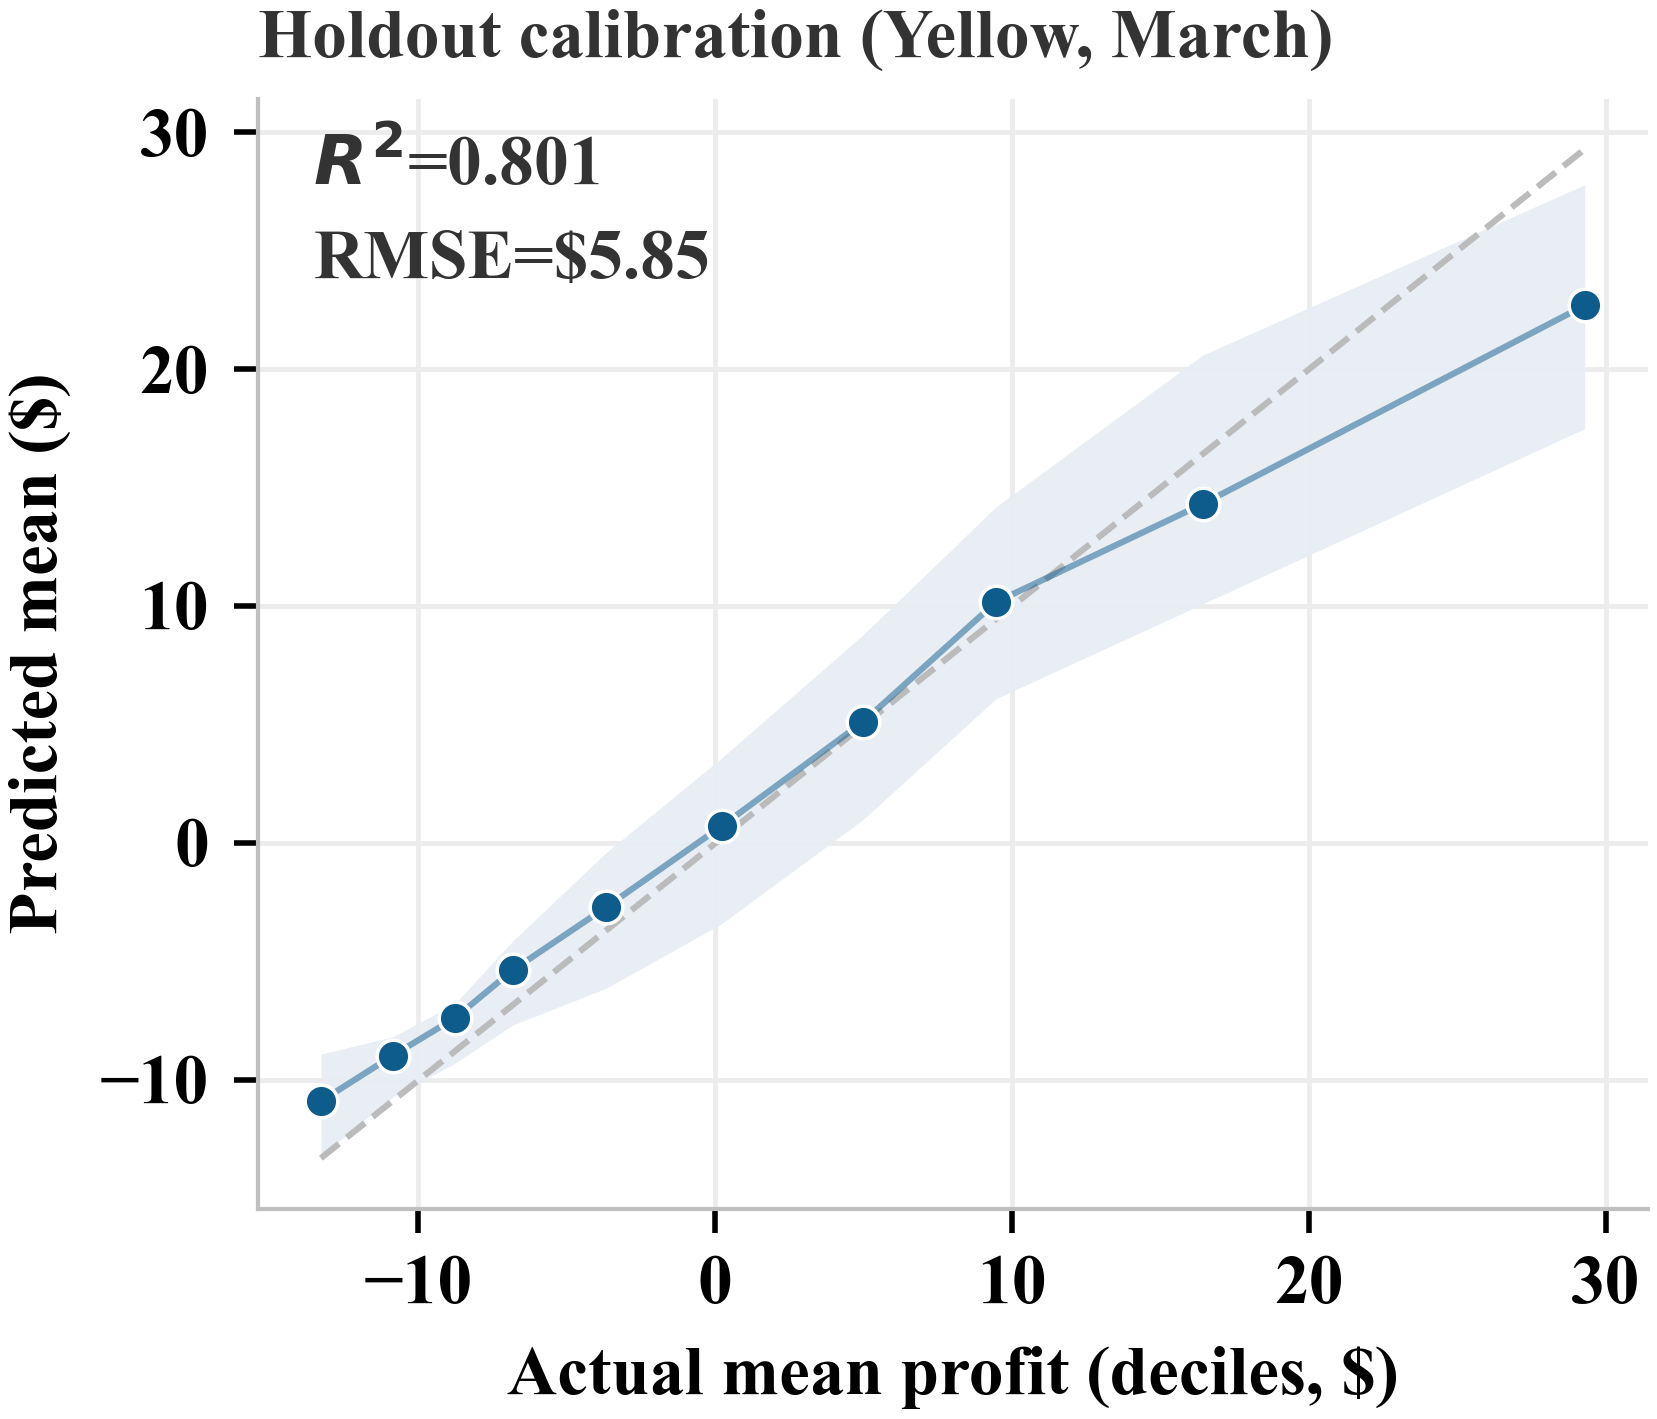
\includegraphics[width=\linewidth]{figures/paper_fig6_model_support.png}
\caption{Holdout calibration for the deployed Yellow LightGBM scorer (March 2015 temporal holdout). Points are decile means of actual versus predicted route profit; the shaded band is the model's interquartile prediction range across routes in each decile. Reported \(R^2\) and RMSE are taken from the model comparison table on the same holdout.}
\label{fig:model_support}
\end{figure}

Figure~\ref{fig:model_support} shows that predicted means track decile-level actual profits on the March holdout without collapsing to a single average, which is the behavior expected of a route scorer used for ranking within a small alternative set. Table~\ref{tab:model_ablation} confirms that removing spatial-demand features causes the largest degradation among the checked ablations. The model therefore appears to learn demand exposure, and the paper presents ML as a residual demand-aware route scorer rather than as the core novelty. Table~\ref{tab:model_policy_diagnostic} adds a narrow policy-level diagnostic across model families on cached held-out route alternatives. It shows that several model families improve over cold-start in route-choice profit, but the ordering is not identical to the full temporal-holdout predictive ranking; this reinforces the conservative decision to avoid claiming that one learner dominates operationally.

\subsection{Sensitivity and Runtime}
Figure~\ref{fig:sensitivity} refines the realism story inside the 10\% stress test. In Yellow dispatch at 10\% density, a tight 2-minute request window with a 2-minute detour yields only \(\$0.36\) of warm-up improvement over cold-start. The primary 5-minute / 4-minute cell yields \(\$0.91\) in the sensitivity grid, consistent with the \(\$0.93\) reported in Table~\ref{tab:dispatch_primary} (the small difference reflects separate seeded runs). A looser 10-minute request window with a 6-minute detour yields \(\$1.36\). Request-window assumptions therefore matter more than moderate detour changes.

\begin{figure}[!t]
\centering
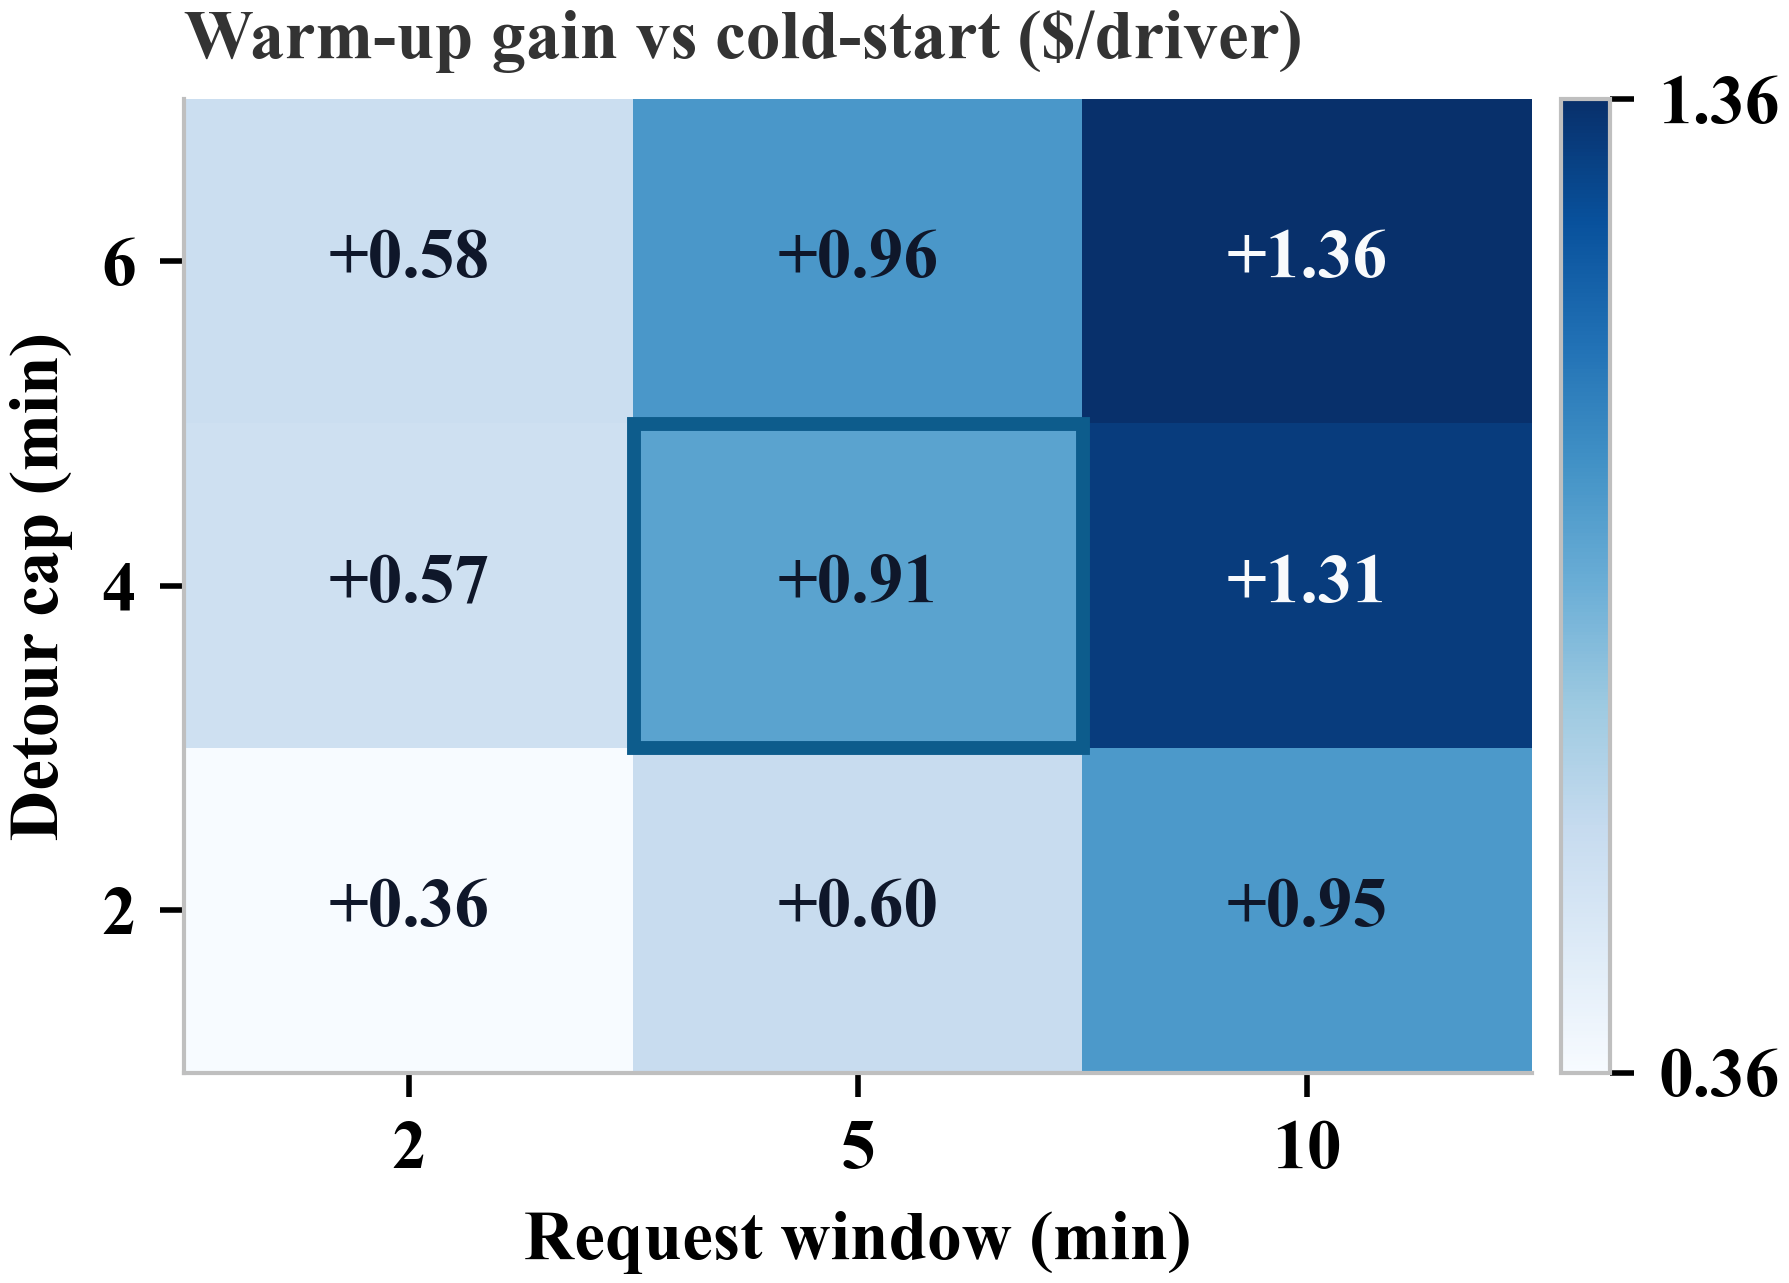
\includegraphics[width=\linewidth]{figures/paper_fig7_sensitivity.png}
\caption{Yellow dispatch sensitivity at 10\% retained-sample density. Each cell reports warm-up improvement over cold-start in scenario profit per launched driver, equivalently the reduction in operating loss. The heatmap shows that request-window assumptions move the dispatch result more than moderate detour relaxation, reinforcing the paper's timing-sensitivity claim.}
\label{fig:sensitivity}
\end{figure}

Retrieval geometry also matters. In the single-driver H3 sensitivity, a coarser H3-8 corridor increases warm-up loss to \(\$8.88\), while a wider two-ring corridor reduces it to \(\$4.91\) but lets the strongest heuristic overtake ML by about \(\$0.05\). A cached dispatch-level corridor diagnostic on 50 April Yellow drivers is summarized in Table~\ref{tab:dispatch_corridor_sensitivity}. This smaller dispatch run recomputes rider H3 cells when the route resolution changes, then reruns the same exact-window and rider-exclusivity logic. The result should be read as a sensitivity diagnostic rather than a replacement for the 1000-driver headline: wider or coarser corridors serve more riders and reduce loss, while increasing route-neighborhood exposure also changes the matching problem being solved.

\begin{table}[!t]
\caption{Cached dispatch-level corridor sensitivity diagnostic for the feasible-count heuristic: Yellow 10\% density, 5-minute request window, 4-minute detour, 50 drivers, one seed.}
\label{tab:dispatch_corridor_sensitivity}
\centering
\scriptsize
\setlength{\tabcolsep}{3.0pt}
\begin{tabular}{|l|r|r|r|}
\hline
Corridor setting & Loss/driver (\$) & Matched/driver & Eval (ms) \\
\hline
H3-9, k=1, 80 m & 7.57 & 0.30 & 39.1 \\
\hline
H3-8, k=1, 80 m & 6.97 & 0.42 & 38.0 \\
\hline
H3-9, k=2, 80 m & 7.18 & 0.40 & 39.6 \\
\hline
H3-9, k=1, 160 m & 7.57 & 0.30 & 35.3 \\
\hline
\end{tabular}
\end{table}

The corridor definition therefore changes both the candidate pool and the difficulty of the route-ranking problem.

Finally, the dispatch layer is lightweight once the route cache is populated. Table~\ref{tab:runtime} reports mean per-driver evaluation time and mean batch runtime for the primary Yellow dispatch scenario. All four reported policies remain around 17.2--17.4 ms per driver and 36.6--37.1 ms per batch on average. We also profiled the route lookup, corridor construction, and candidate filtering/matching stages on 100 cached multi-route April Yellow drivers. Table~\ref{tab:end_to_end_runtime} reports a mean cached route-scoring path of 13.1 ms and a worst profiled path of 66.2 ms. The Yellow route cache used in the path-buffer comparison has 1000 route entries, and scan misses in this profile reflect candidate-level route-screening probes against the reproducibility cache rather than a production cache hit-rate claim. The resource audit reports a 23.1 MB SQLite route-cache footprint, 22.8 kB average route payload, and 0.13 MB traced Python allocation for opening the cache and reading one route entry; the cache is not loaded wholesale into memory. As a separate network diagnostic, five uncached public OSRM requests averaged 1.68 s, with 1.78 s median latency and mean 1.6 returned alternatives; this public-server probe is not a production latency guarantee.

\begin{table}[!t]
\caption{Primary Yellow dispatch runtime. Times exclude live OSRM fetch latency because the simulator runs against the cached route store.}
\label{tab:runtime}
\centering
\scriptsize
\setlength{\tabcolsep}{4.0pt}
\begin{tabular}{|l|r|r|}
\hline
Policy & Mean eval (ms) & Mean batch (ms) \\
\hline
Cold-start & 17.3 & 36.9 \\
\hline
Best heuristic & 17.4 & 37.1 \\
\hline
ML warm-up & 17.3 & 36.9 \\
\hline
Oracle (route set) & 17.2 & 36.6 \\
\hline
\end{tabular}
\end{table}

\begin{table}[!t]
\caption{Cached end-to-end route-scoring profile on 100 cached multi-route April Yellow drivers.}
\label{tab:end_to_end_runtime}
\centering
\scriptsize
\setlength{\tabcolsep}{3.6pt}
\begin{tabular}{|l|r|r|r|r|}
\hline
Statistic & Cache lookup & Corridor build & Filter/match & Total \\
\hline
Mean ms & 1.3 & 5.0 & 6.7 & 13.1 \\
\hline
Median ms & 1.4 & 4.9 & 6.0 & 11.6 \\
\hline
Max ms & 2.7 & 48.2 & 19.3 & 66.2 \\
\hline
\end{tabular}
\end{table}

\section{Discussion}
The experiments support three bounded conclusions.

First, route-aware candidate construction changes the dispatch comparison. After exact request-window filtering and rider exclusivity, the route-aware policies reduce operating loss relative to default cold-start routing in both Yellow and Green. Route choice therefore changes which riders are matchable under the stated timing and detour rules.

Second, learned route ranking is useful but not dominant once strong heuristics are already in place. In the primary Yellow sparse scenario, ML warm-up improves upon the strongest heuristic by \(\$0.15\) per launched driver; in Green the corresponding margin is \(\$0.27\). The single-driver and dispatch decompositions give the same interpretation: most of the route-aware gain is recovered by heuristic route choice, leaving ML to capture a smaller residual layer of value.

Third, exact timing is a methodological lever, not a bookkeeping detail. The sensitivity analysis shows that request-window assumptions shift results more than moderate detour relaxation. This implies that ride-pooling studies should distinguish retrieval acceleration tricks from the actual matching rule. In the present implementation, H3 corridors and 15-minute bins narrow the search; exact timestamp compatibility determines which riders remain eligible.

The path-buffer sanity baseline also clarifies the retrieval claim. A 1 km geometric buffer around the route recovers some candidate overlap, but it does not approach the matching-ball policies under the same timing and feasibility rules. The difference indicates that the value is not simply ``using more geometry,'' but using route-specific corridor construction that is explicit about both pickup and drop-off compatibility before scoring.

The study remains bounded. It is an offline proxy design based on taxi trajectories rather than native pooled requests, so the public benchmark should be read as a controlled test of route-aware candidate construction rather than as a replica of live pooled-demand behavior. The dispatch simulator is rolling-horizon and exclusivity-aware but does not model repositioning or full many-driver global assignment. The public second domain, NYC Green, is a same-city service-type check, not a substitute for a true second city or restricted operator dataset. The dispatch study uses 1000 drivers and five seeds, which is sufficient for the present comparative evidence but not for a full-scale deployment claim. Finally, the reported losses and loss reductions are scenario-based operating metrics under fixed share and cost assumptions rather than calibrated financial forecasts.

These constraints narrow the paper's scope. The paper does not claim that a learned route scorer solves dispatch. It shows that route-aware matching-ball retrieval and exact-time eligibility change route-selection conclusions in this public-data proxy, and that strong non-ML heuristics remain the relevant benchmark for learned ranking in shared dispatch environments.

\section{Code and Reproducibility}
The research code is maintained at \url{https://github.com/kaushik-kamuit/R-D-1}. The public repository includes the manuscript source, route-cache-aware scripts, summary tables, figure-generation scripts, and consistency validation. The repository README and \texttt{paper/README.md} list the commands used to regenerate the main results, including the stronger-baseline, path-buffer, OSRM-latency, runtime-resource, model-policy, validation-heuristic, dispatch-corridor, dispatch-gap, dispatch-uncertainty, and paper-consistency scripts. Route caches are stored as SQLite files under \texttt{data/route\_cache\_<domain>.db}; the Yellow route cache used by the path-buffer comparison contains 1000 entries after live-or-cached route expansion.

\section{Conclusion}
This paper evaluates route-aware warm-up for ride-pooling in a public taxi proxy. The method is a matching-ball retrieval layer built from H3 corridors, exact request-time filtering, feasibility checks, and route ranking over genuine OSRM alternatives. Embedded inside a rolling-horizon dispatch simulator, the route-aware layer reduces operating loss relative to cold-start routing in the Yellow sparse scenario and preserves the same policy ordering in the Green same-city service-type check.

The controlled paired study clarifies the mechanism behind the dispatch result. Strong heuristics recover most of the route-aware gain in both isolated and shared settings, while learned route ranking contributes a smaller residual improvement. The paper therefore contributes a route-aware candidate-construction method and an evaluation protocol for route-selection policies under exact timing assumptions.

The methodological implication is direct: ride-pooling studies should not conflate coarse retrieval bins with request compatibility, and they should treat route choice as part of candidate construction rather than as a downstream routing detail. Future work should test the same mechanism with larger dispatch studies, additional public markets or restricted operational data, and richer many-driver assignment and repositioning logic.

\bibliographystyle{IEEEtran}
\bibliography{references}

\end{document}
